\chapter{SAF microarchitecture conceptual framework}
\label{chapter:conceptual_framework}

The \textit{Efficient Processing} framework presents a consistent set of abstractions for describing the impact of sparsity on microarchitecture. However, as discussed in Section~\ref{chapter:introduction} the goal of this work is to create a framework for defining SAF microarchitectures at a fine enough granularity to enable modeling and comparison between designs, while still keeping the framework general enough to describe a wide range of designs. A few challenges that come with applying the \textit{Efficient Processing} SAF microarchitecture taxonomy to this problem are

\begin{itemize}
    \item The components in the \textit{Efficient Processing} SAF microarchitecture taxonomy are black boxes without any associated models of area, actions, or energy. This makes evaluation or comparison of design choices more time-consuming because models must be designed from scratch.
    \item Among the \textit{Efficient Processing} primitives there is wide variation in complexity. Intersection units, position generators, and coordinate generators, for example, are relatively simple components. In contrast, the \textit{Efficient Processing} taxonomy also includes (for example) a number of different types of memories - in practice, memories may vary wildly in terms of i.e. what type of memory is employed (SRAM, DRAM, register file, etc.), how data orchestration is handled, what special features are supported (i.e. error correction), etc. Additionally, because the \textit{Efficient Processing} strives to show that sparse dataflows may be conceptually mapped to dataflow microarchitectures, microarchitecture designs created using the \textit{Efficient Processing} taxonomy are relatively complex.
    \item While it is helpful to have a consistent set of SAF microarchitecture abstractions that are decoupled from the fine details of manipulating sparse representation formats, this means that the co-design process will eventually run up against the difficulty of going from a high-level SAF microarchitecture topology built out of \textit{Efficient Processing} primitives, to a more fleshed-out design that is compatible with the sparse representation formats used to compress the operands.
    
\end{itemize}

Building on the \textit{Efficient Processing} SAF microarchitecture topology, this work applies three strategies to address the above challenges: 

\begin{itemize}
    \item Shrink the SAF microarchitecture design-space, by decoupling SAF microarchitecture from architecture and dataflow.
    \item Augment \textit{Efficient Processing} microarchitecture primitives with \textit{parameterization} and \textit{composition}. While the existing \textit{Efficient Processing} taxonomy is good for describing a \textit{format-agnostic} SAF microarchitecture, parameterization and composition will enable a systematic process for deriving an elaborated SAF microarchitecture that is \textit{co-designed} for dataflow and sparse representation format.
    \item Associate each SAF microarchitecture primitive with an analytical cost model, enabling evaluation and comparison between designs.
\end{itemize}

% Extending Efficient Processing framework

% Decoupling SAF microarchitecture from dataflow
% - Narrower definition of SAF microarchitecture
% - => Coupled access
% - Managing SAF microarchitecture/representation format co-design through parameterization
% - => Parameterization for capturing additional design flexibility
% - Decoupling from dataflow through boundary conditions
% - => High-level intro
% - Additional notes on prior work
% - => Skipping topologies & always having pgen
% - => Pgen reference
% - => Fill optimizers
% - Overview of proposed conceptual framework
% - => Buffer model & format interfaces
% - => Workload modeling
% - => SAF uarch component - fmt- and dataflow-indep
% - => Taxo of parameterized primitives & models
% - => 

Starting from these principles, this section shows builds up a conceptual framework based on these three strategies, making sure to integrate insights from prior work on sparse tensor accelerators.

\section{Decouple SAF microarchitecture from architecture and dataflow}
\label{sec:what_is_a_saf_microarchitecture}

\textit{Efficient Processing} attempts to design a rough correspondence between sparse dataflow loop nests, and microarchitectural topologies\cite{szebook}. However, in this work, the correspondence between sparse loop nests and microarchitectural topologies is eschewed in favor of focusing on \textit{the correspondence between the Sparseloop\cite{sparseloop} SAF declaration, and the underlying SAF microarchitecture.} Note that a Sparseloop SAF carries no information about dataflow. This change of focus permits us to sharply delineate what qualifies as a SAF microarchitecture component:

\begin{itemize}
    \item If a microarchitectural component or circuit is introduced by an author with the explicit goal of allowing a design to exploit sparsity in some way, that is a SAF microarchitecture.
    \item A microarchitectural component which, if removed or replaced with a naive implementation, would render the accelerator unable to cope with traversing, co-iterating, or otherwise working with sparse representation formats, is a SAF microarchitecture.
\end{itemize}

What is \textit{not} a SAF microarchitecture:

\begin{itemize}
    \item Any architectural component - buffer, compute, etc. - is not SAF microarchitecture.
    \item Any microarchitecture which is not unique to sparse tensor accelerators, is not SAF microarchitecture (i.e. the microarchitectural details of switches within a NoC, unless there are \textit{specific optimizations for network routing in the presence of sparsity}, do not comprise SAF microarchitecture)
    \item In this work \textit{dataflow} is conceived of as something that architecture \textit{does}; since architecture is excluded from SAF microarchitecture, any logic which implements dataflow is by default not SAF microarchitecture. This excludes, for example, most address generators or sequence generators, such as the \textit{Efficient Processing} position generator and coordinate generator components. However, microarchitectures which implement dataflow \textit{in a specific fashion to account for sparsity}, would count as SAF microarchitecture.
\end{itemize}

\subsection{Sequence generators and decoupled orchestration}

\textit{Efficient Processing}\cite{szebook} primarily focuses on describing EDDO\cite{buffet} accelerators; thus, the \textit{position generator} and \textit{coordinate generator} components in the \textit{Efficient Processing} taxonomy serve to implement EDDO dataflows, by generating pre-determined sequences of position or coordinate values, respectively.

Thus, we will refer to these components as \textit{decoupled} position generators and \textit{decoupled} coordinate generators, respectively.

Later in this section we will explore a \textit{coupled} position generator, which outputs position offsets that are a function of metadata values passed in as inputs (i.e. memory loads triggered by the coupled pgen, are coupled to metadata values generated by another component.) Since as we will see, coupled position generators are introduced expressly for the purpose of implementing SAFs, therefore coupled position generators are automatically a type of SAF microarchitecture component, as reflected in Table~\ref{tab:reclassify_saf_microarchitecture}.

Going forward, this work assumes that all architectural memories are \textit{smartbuffers}\cite{smartbuffer}, memories with integrated logic for decoupled traversal of stored tensors.

A theme of this work is that sparsity and coupled data ochestration may go hand-in hand. One could argue that the EDDO classification applies only loosely to the sparse smartbuffers explored in this work: as we will see, SAFs such as skipping cause the sequence of payload accesses to be conditional and non-deterministic, i.e. based on the pattern of intersections between two sparse fibers. Going forward, this work uses EDDO to describe smartbuffers which are ``loosely EDDO'', i.e. the smartbuffer supports EDDO for reading sparse format metadata, but may (or may not) allow SAF microarchitecture to trigger coupled payload reads as a consequence of metadata parsing or of intersecting sparse format metadata from two fibers.

\subsection{Reclassifying the \textit{Efficient Processing} taxonomy}

Table~\ref{tab:reclassify_saf_microarchitecture} reclassifies the \textit{Efficient Processing} taxonomy in Figure~\ref{fig:efficient_processing_taxo} based on the aforementioned more-stringent criteria for what qualifies as SAF microarchitecture.

\begin{table}
\centering
\caption{Reclassification of \textit{Efficient Processing}\cite{szebook} primitives}
\label{tab:reclassify_saf_microarchitecture}
\begin{tabular}{||p{0.3\textwidth}|l|l||}\hline
\textbf{SAF $\mu$arch} & \textbf{Non-SAF $\mu$arch} & \textbf{Architecture}  \\\hline
Intersection & \textit{Decoupled} pgen & Uncompressed data buffer \\\hline
\textit{Coupled} pgen & \textit{Decoupled} cgen & Updating uncompressed data buffer \\\hline
Support for coordinate calculations against sparse formats & Coordinate calculator & Compressed data buffer \\\hline
 &  & Latch \\\hline
 &  & MAC \\\hline
\end{tabular}
\end{table}

Some observations about this reclassification:
\begin{itemize}
    \item Most of the \textit{Efficient Processing} taxonomic primitives are reclassified as architecture or non-SAF microarchitecture, and thus will not be part of the taxonomy developed in this work.
    \item Note that coordinate arithmetic units are classified as ``non-SAF microarchitecture'' because dense accelerators also perform coordinate arithmetic, so we assume here that existing tools are frameworks handle coordinate arithmetic well enough that we need not consider \textit{the coordinate arithmetic itself.}
    \item That said, to perform coordinate arithmetic on coordinates traversed by some rank $i$, requires that \textit{explicit}\cite{szebook} coordinate values be available as that rank is traversed - something which is not automatically true i.e. of implicit coordinate sparse representation formats, such as bitmask (B)\cite{szebook}. The need to extract explicit coordinates from implicit coordinate metadata solely to facilitate coordinate arithmetic, only arises in the context of a sparse tensor accelerator; thus, Table~\ref{tab:reclassify_saf_microarchitecture} classifies logic which supports coordinate arithmetic for implicit coordinate fibers as SAF microarchitecture.
\end{itemize}

\section{Decoupling SAF microarchitecture from dataflow via \textit{workload boundary conditions}}

In this work, the key to decoupling dataflow from SAF microarchitecture modeling is to encapsulate memory internals inside an abstract smartbuffer with a format-agnostic interface (Figure~\ref{fig:sparse_sbuff_overview}.) 

\begin{figure}[ht]
    \centering
    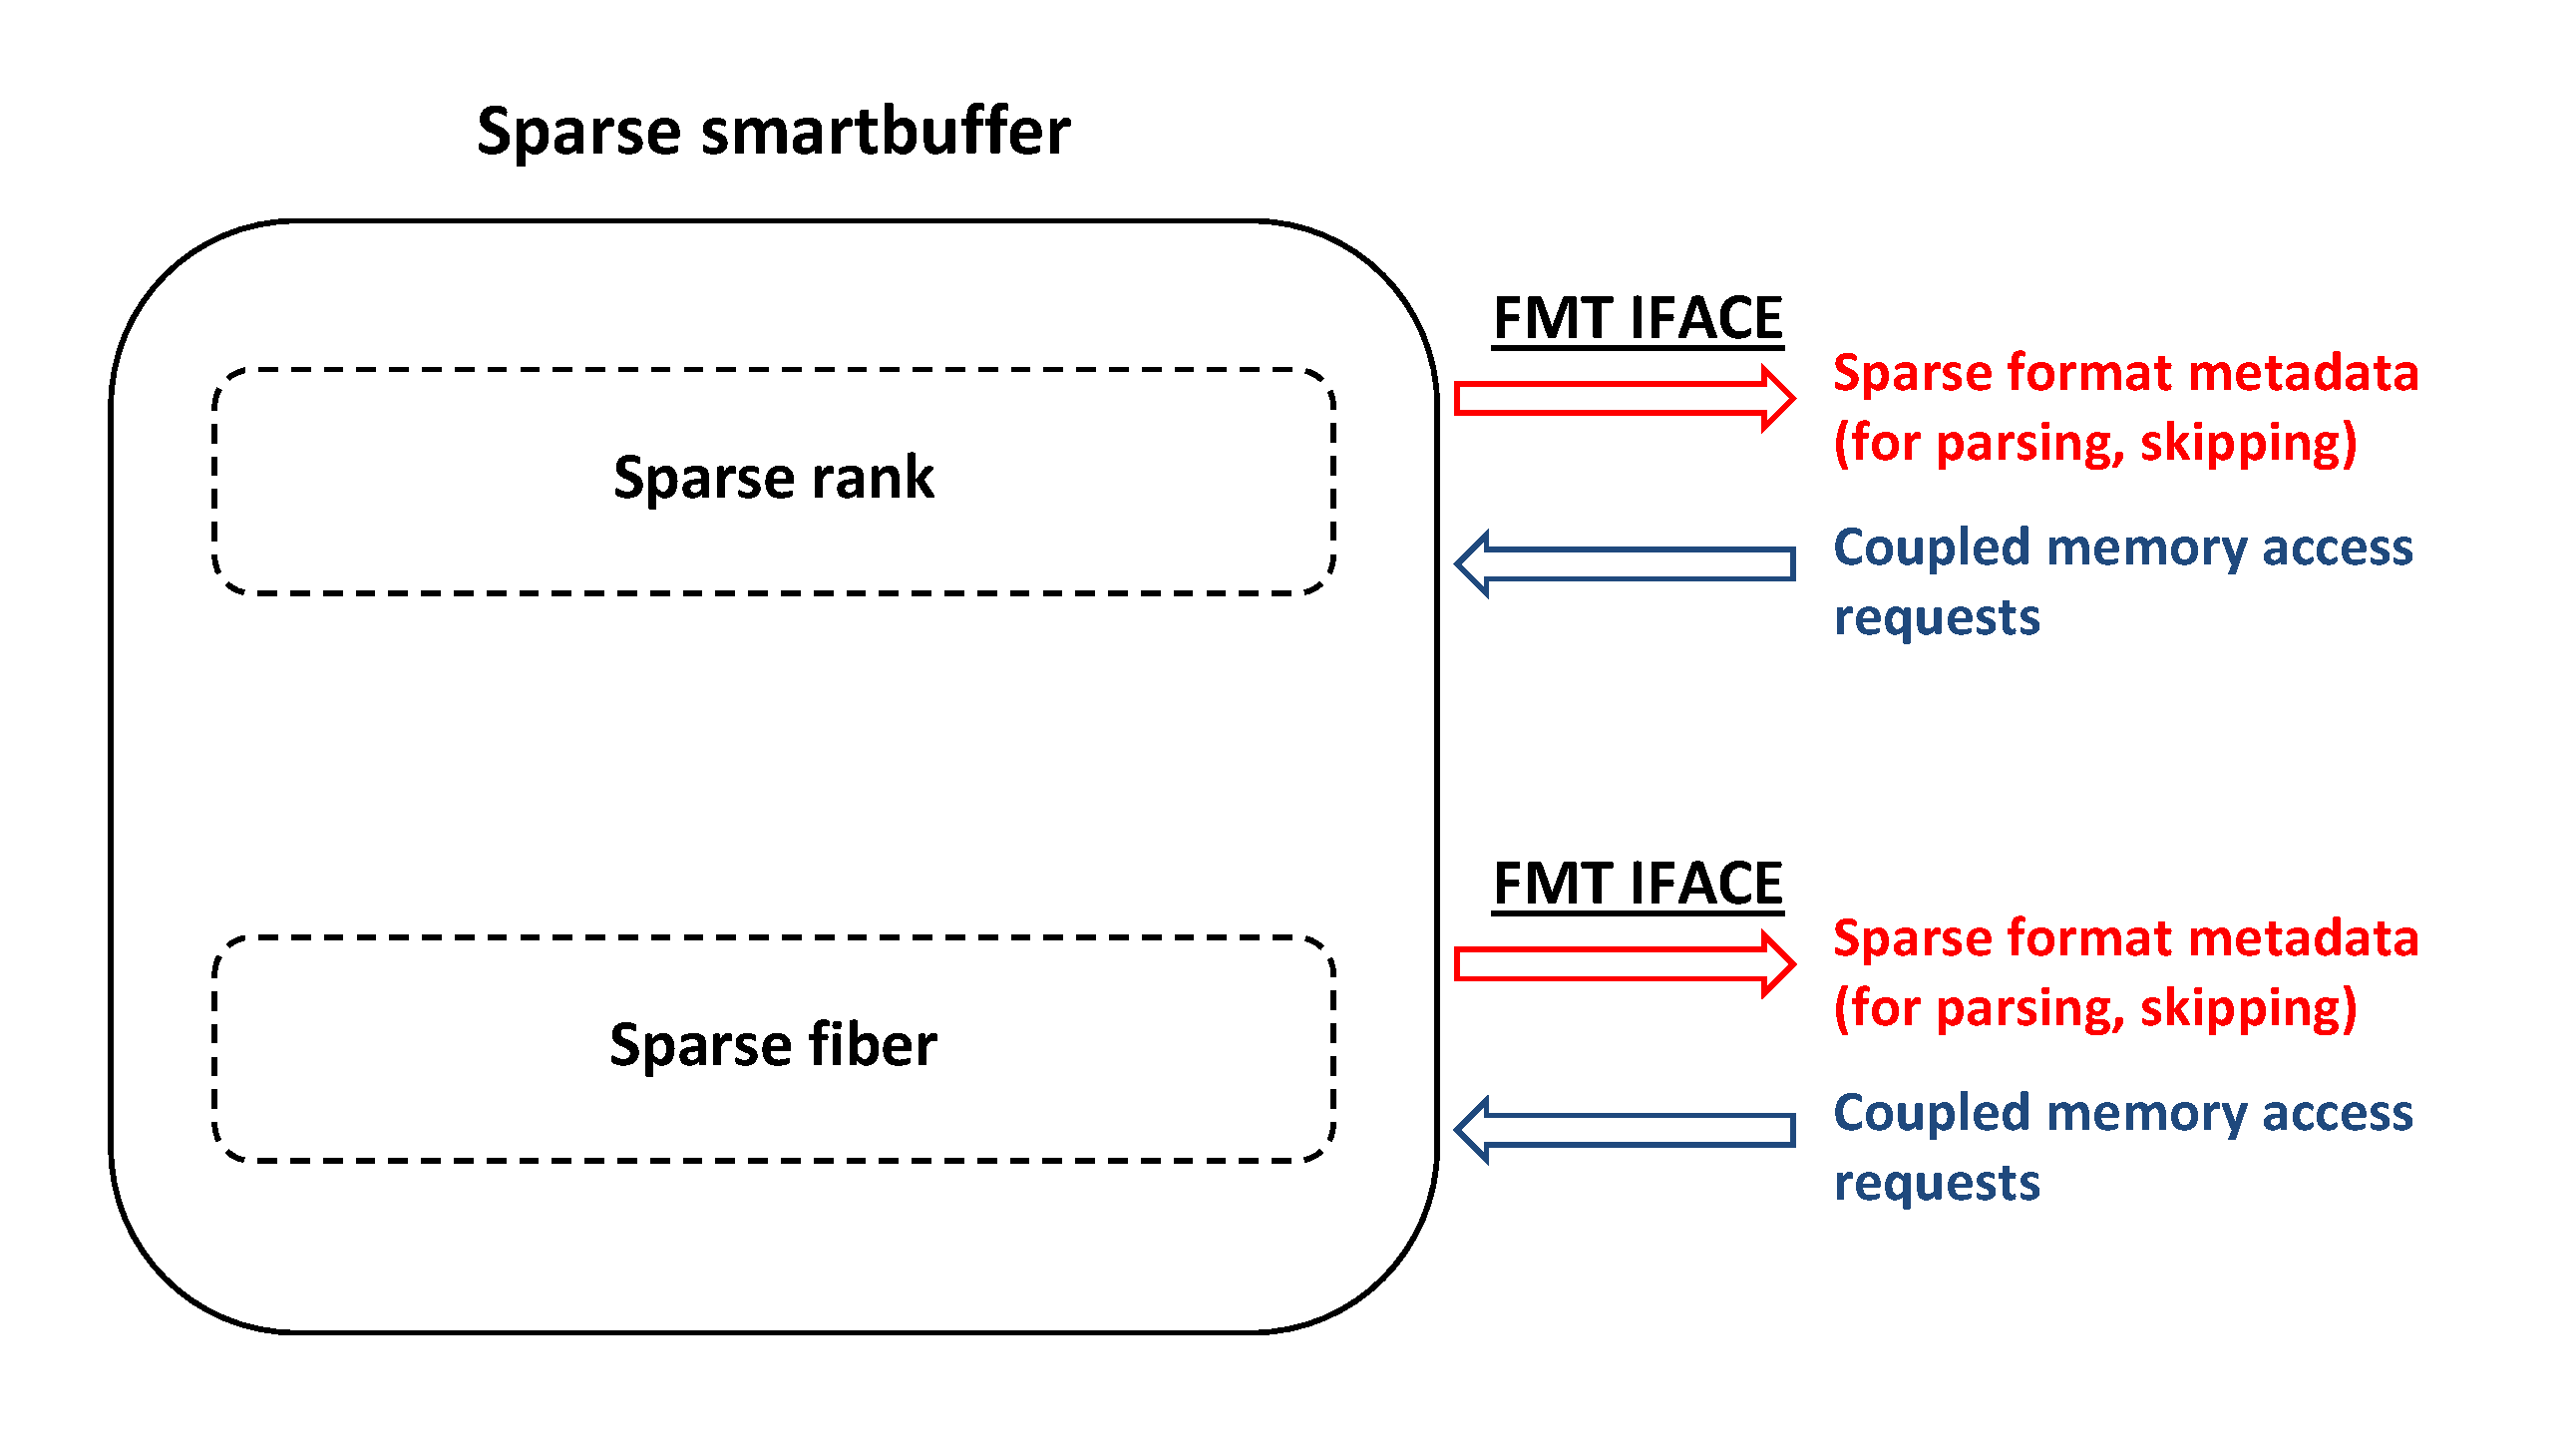
\includegraphics[width=0.95\textwidth]{figures/sparse_sbuff_overview.pdf}
    \caption{In this work, the details of memory implementation are encapsulated inside an abstract ``sparse smartbuffer'' with an identical IO bundle interface to each sparse rank. SAF microarchitecture can read a sparse fiber's format metadata from the format interface, and can also write to the format interface in order to trigger a payload read from a specified positional offset within the same sparse fiber.}
    \label{fig:sparse_sbuff_overview}
\end{figure}

Each fibertree rank resident in the buffer is hidden behind a format-agnostic IO bundle, called the ``format interface'' (fmt iface.) The format interface supports three operations:

\begin{itemize}
    \item \textbf{Get sparse fiber metadata:} Read a stream of sparse format metadata associated with one fiber in a given rank.
    \item \textbf{Request payload read at specified positional offset:} Coupled data orchestration is supported via input wires in the format interface IO bundle, which allow SAF microarchitecture to override the smartbuffer's internal decoupled data orchestration. Where EDDO data orchestration is desired, the format interface IO bundle inputs can simply be left unconnected.
    \item \textbf{Signal end-of-fiber:} Although \textit{Efficient Processing}\cite{szebook} focuses on EDDO data orchestration, some sparse dataflow microarchitectures proposed in the book have a limited amount of coupled data orchestration, in the form of one-bit flags which synchronously reset the otherwise decoupled sequence generators when the end of a fiber is reached. In this work, the format interface IO bundle includes a flag for signaling that the end of a fiber has been reached. The assumption here is that recognizing the end of a fiber may require specialized format metadata parsing within the SAF microarchitecture, and thus the format interface requires a flag input for the SAF microarchitecture to signal end-of-fiber to the rank's decoupled traversal logic.
\end{itemize}

Note the particular usage of ``encapsulation'' in this work: for the purposes of describing and modeling SAF microarchitecture, the internals of each sparse smartbuffer are not simply hidden behind the format interface, but rather are not implemented or modeled at all. The goal instead is to (1) define a consistent abstraction for the interface between architectural smartbuffers and SAF microarchitecture, and (2) define a set of \textit{workload boundary conditions} which are \textit{consistent} with sparse smartbuffer functionality under worst-case dataflow conditions. Here, \textit{workload} refers to any appropriate measure of the processing effort that is required of a SAF microarchitecture connected to the IO. Once the worst-case workload requirements are estimated for all format interfaces, then the SAF microarchitecture may be designed to satisfy the workload requirements, without regard to the overall dataflow. 

Figure~\ref{fig:sparse_sbuff_wkld_overview} provides a high-level overview of how workload boundary conditions are bound to format interfaces on a sparse smartbuffer. Note that all workload measures have a \textit{direction} which matches the IO they apply to. In Figure~\ref{fig:sparse_sbuff_wkld_overview}, the $w_{md}$ workloads (red) are bound to format interface output wires; $w_{md}$ is a measure of the processing effort imposed on the \textit{input port} of any SAF microarchitecture connected to the format interface output wires. The $w_{pos}$ workloads (blue) are bound to format interface input wires; $w_{pos}$ is a measure of the processing effort imposed on the \textit{output port} of any SAF microarchitecture connected to the format interface input wires.

\begin{figure}[ht]
    \centering
    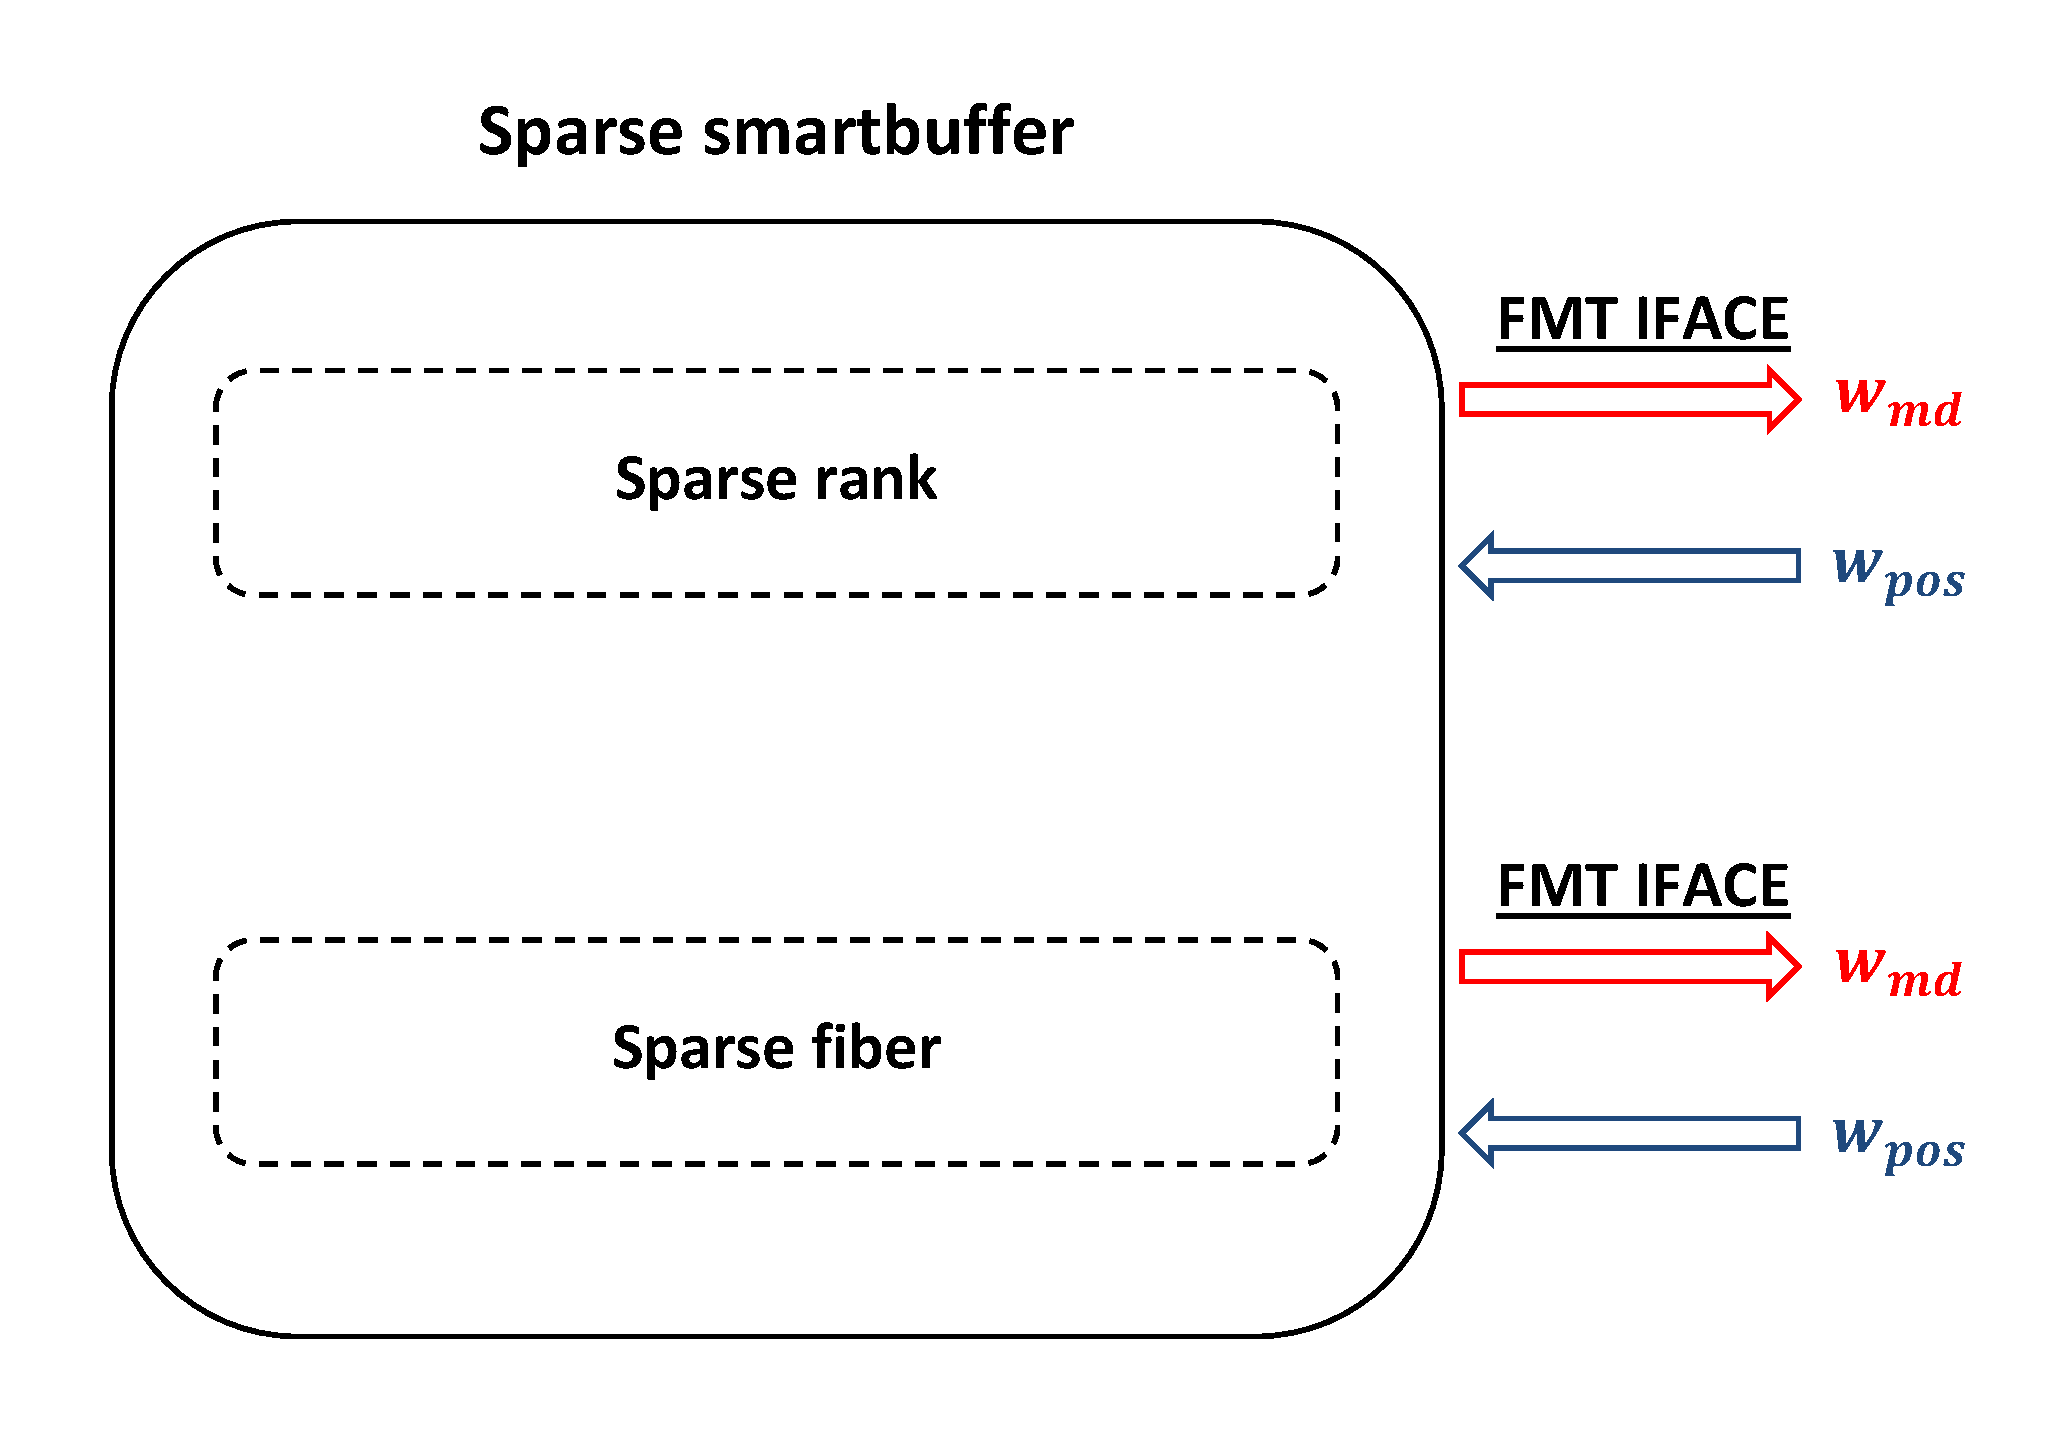
\includegraphics[width=0.95\textwidth]{figures/sparse_sbuf_wkld_overview.pdf}
    \caption{Sparse dataflow is abstracted behind \textit{workload boundary conditions}}.
    \label{fig:sparse_sbuff_wkld_overview}
\end{figure}

% Architecture, non-SAF microarchitecture, SAF microarchitecture



\subsection{Sparse smartbuffer model}

Although this work is not focused on modeling sparse smartbuffers, nonetheless it is helpful to develop a ``reference design'' for what a sparse smartbuffer implementation might look like. There are two reasons for this

\begin{itemize}
    \item \textbf{Define the format interface IO bundle.} Creating a sparse smartbuffer reference design helps us to be very concrete about what input and output wires a format interface must have, in order to support the most common workloads that operate on sparse fibers.
    \item \textbf{Workload modeling.} A mental model of sparse smartbuffer internals will be helpful later on when we bind workload measures to format interfaces.
\end{itemize}

This section will build up a reference design for a sparse smartbuffer in steps: (1) describe a single-fiber sparse smartbuffer for explicit-coordinate representation formats, (2) describe a single-fiber sparse smartbuffer for general explicit/implicit coordinate representation formats, and finally (3) describe a pipelined sparse smartbuffer capable of traversing a fibertree with support for general explicit/implicit coordinate representation formats.

\subsubsection{Composition}
\label{sec:composition}

A sparse smartbuffer can utilize some components which are familiar from dense smartbuffers\cite{buffet}\cite{sparseloop}, however, the sparse smartbuffer must have additional logic for operating on sparse fibers in order to correctly traverse a sparse fiber. Recall from Section~\ref{sec:what_is_a_saf_microarchitecture} that a SAF microarchitecture refers to that subset of an accelerator's microarchitecture, which either (1) was designed for processing sparse representation formats, or (2) is critical for the accelerator to correctly process sparse representation formats. This work is focused on describing and modeling SAF microarchitectures; since we ultimately are not striving to model smartbuffer internals, it is desirable to completely decouple the smartbuffer's sparse format processing logic into a separate component.

\begin{figure}[ht]
    \centering
    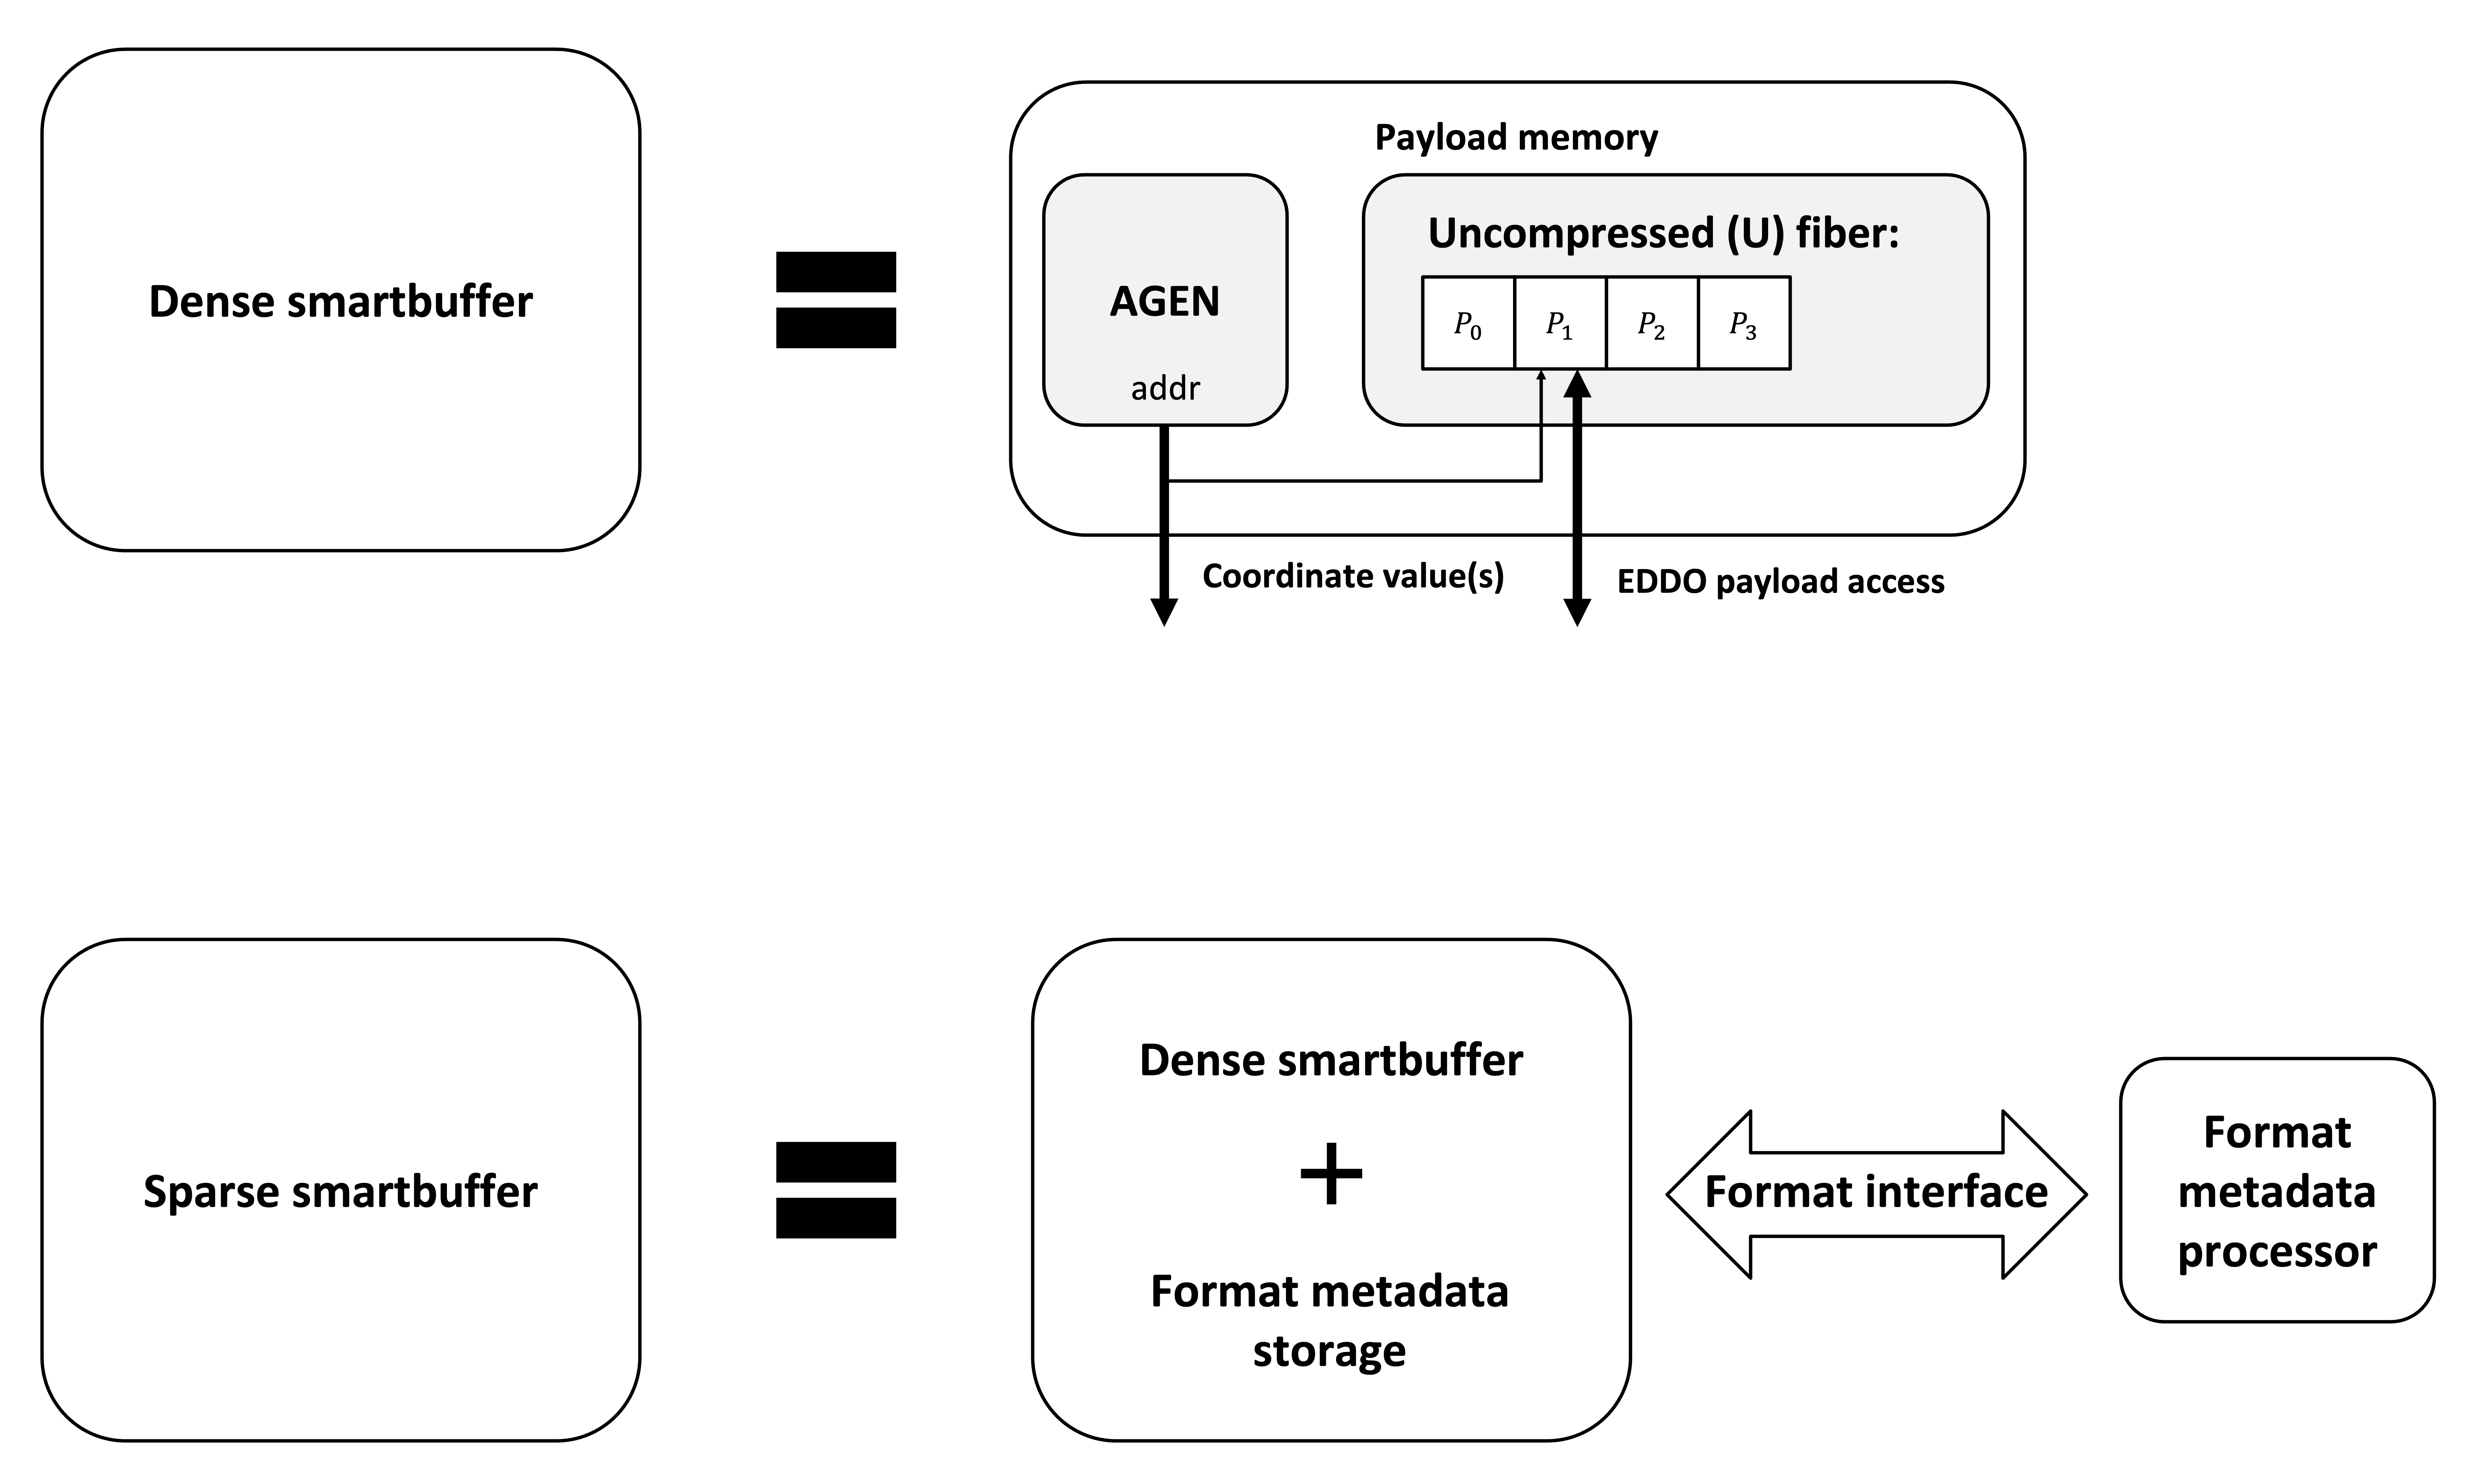
\includegraphics[width=0.95\textwidth]{figures/dense_smartbuffer_composition.png}
    \caption{This work models a \textit{sparse smartbuffer} as the composition of a dense smartbuffer with additional hardware that handles the compressed sparse tensor format, connected by an I/O bundle (``format interface''.) The format interface moves sparse format metadata from the dense smartbuffer metadata storage to the format metadata processor, and moves control signals in the other direction.}
    \label{fig:dense_smartbuffer_composition}
\end{figure}

Figure~\ref{fig:dense_smartbuffer_composition} (\textit{bottom}) shows how the sparse smartbuffer is modeled as a dense smartbuffer (\textit{top}) composed with (1) additional storage for sparse format metadata, and (2) a SAF microarchitecture that can process sparse format metadata. 

The dense smartbuffer in Figure~\ref{fig:dense_smartbuffer_composition} (\textit{top}) only holds one fiber; the AGEN unit implements decoupled fiber traversal by generating a stream of coordinate values which lookup into the uncompressed fiber (position and coordinate are synonymous for an uncompressed fiber.)

When the smartbuffer is storing a compressed sparse fiber, it becomes reliant on the SAF microarchitecture to receive sparse format metadata that is output through the format interface, and to send back control signals which ensure correct traversal.

\subsubsection{Single-rank, explicit-coordinate-format sparse smartbuffer model}
\label{sec:single_explicit_fiber}

Building on Section~\ref{sec:composition}, we can flesh out how the sparse smartbuffer internals and the format interface might be designed if the sparse fiber uses an explicit coordinate\cite{szebook} format such as coordinate-payload (C)\cite{szebook}.

\begin{figure}[ht]
    \centering
    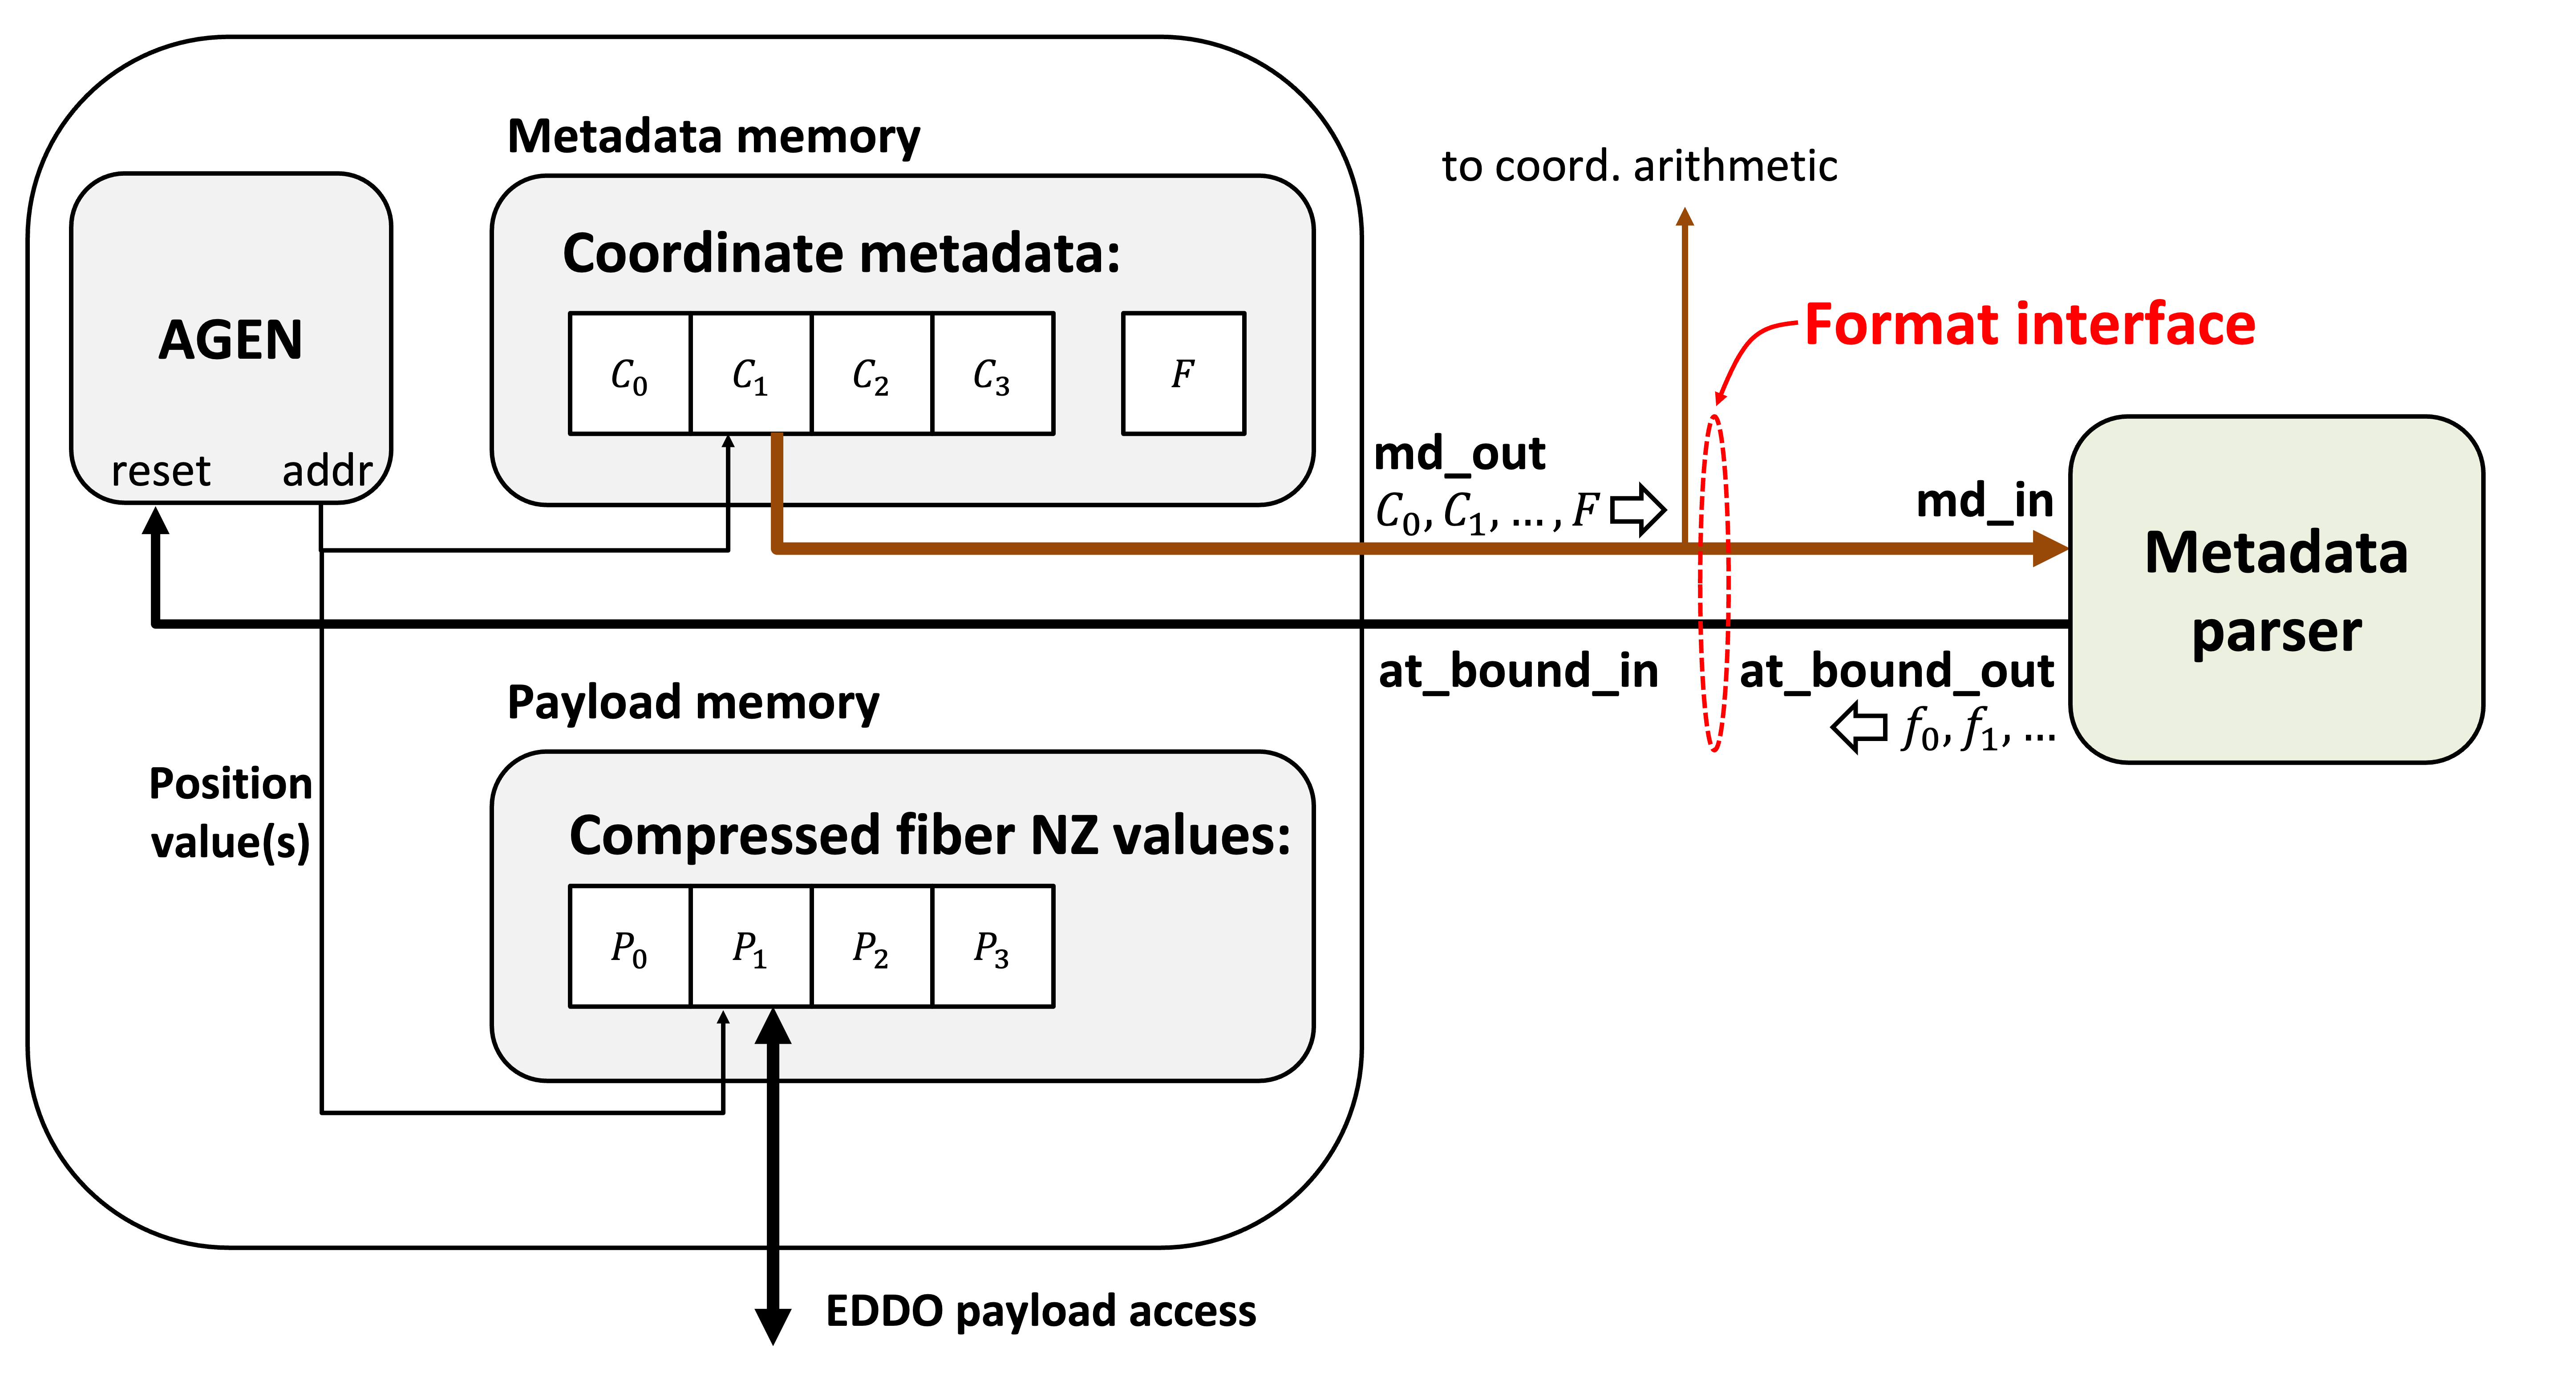
\includegraphics[width=0.95\textwidth]{figures/single_rank_explicit_coordinate_smartbuffer_model.png}
    \caption{Sparse smartbuffer model for a single rank, supporting explicit coordinate sparse tensor formats. ${C_i}$ are explicit coordinate metadata values. $F$ is a stand-in for any metadata regarding fiber characteristics, i.e. number-of-non-zeros. ${f_i}$ are flag values - metadata parser parses metadata arriving at md\_in and sets at\_bound\_out when fiber traversal is complete.}
    \label{fig:single_rank_explicit_coordinate_smartbuffer_model}
\end{figure}

In the coordinate-payload format, each non-zero/non-empty payload is paired with a coordinate metadata value. Figure~\ref{fig:single_rank_explicit_coordinate_smartbuffer_model} shows how the address generator implements traversal by looking up corresponding elements in the \textit{coordinate metadata} and \textit{compressed fiber non-zero (NZ) values} arrays. 

The only role for the metadata parser is to detect when the entirety of the fiber has been processed, and send a reset signal back over the format interface in order reset the traversal. Thus, the format interface consists simply of

\begin{itemize}
    \item \textbf{md\_out (output):} Output a stream of explicit coordinates to the metadata parser.
    \item \textbf{at\_bound\_in (input):} Receive the reset signal from the metadata parser upon completing fiber traversal.
\end{itemize}

\subsubsection{Single-rank, general-format sparse smartbuffer model}

It becomes apparent that the format interface and reference design in Section~\ref{sec:single_explicit_fiber}, while sufficient for an explicit-coordinate sparse format, are insufficient for an implicit-coordinate sparse format such as bitmask (B)\cite{szebook}.

\begin{figure}[ht]
    \centering
    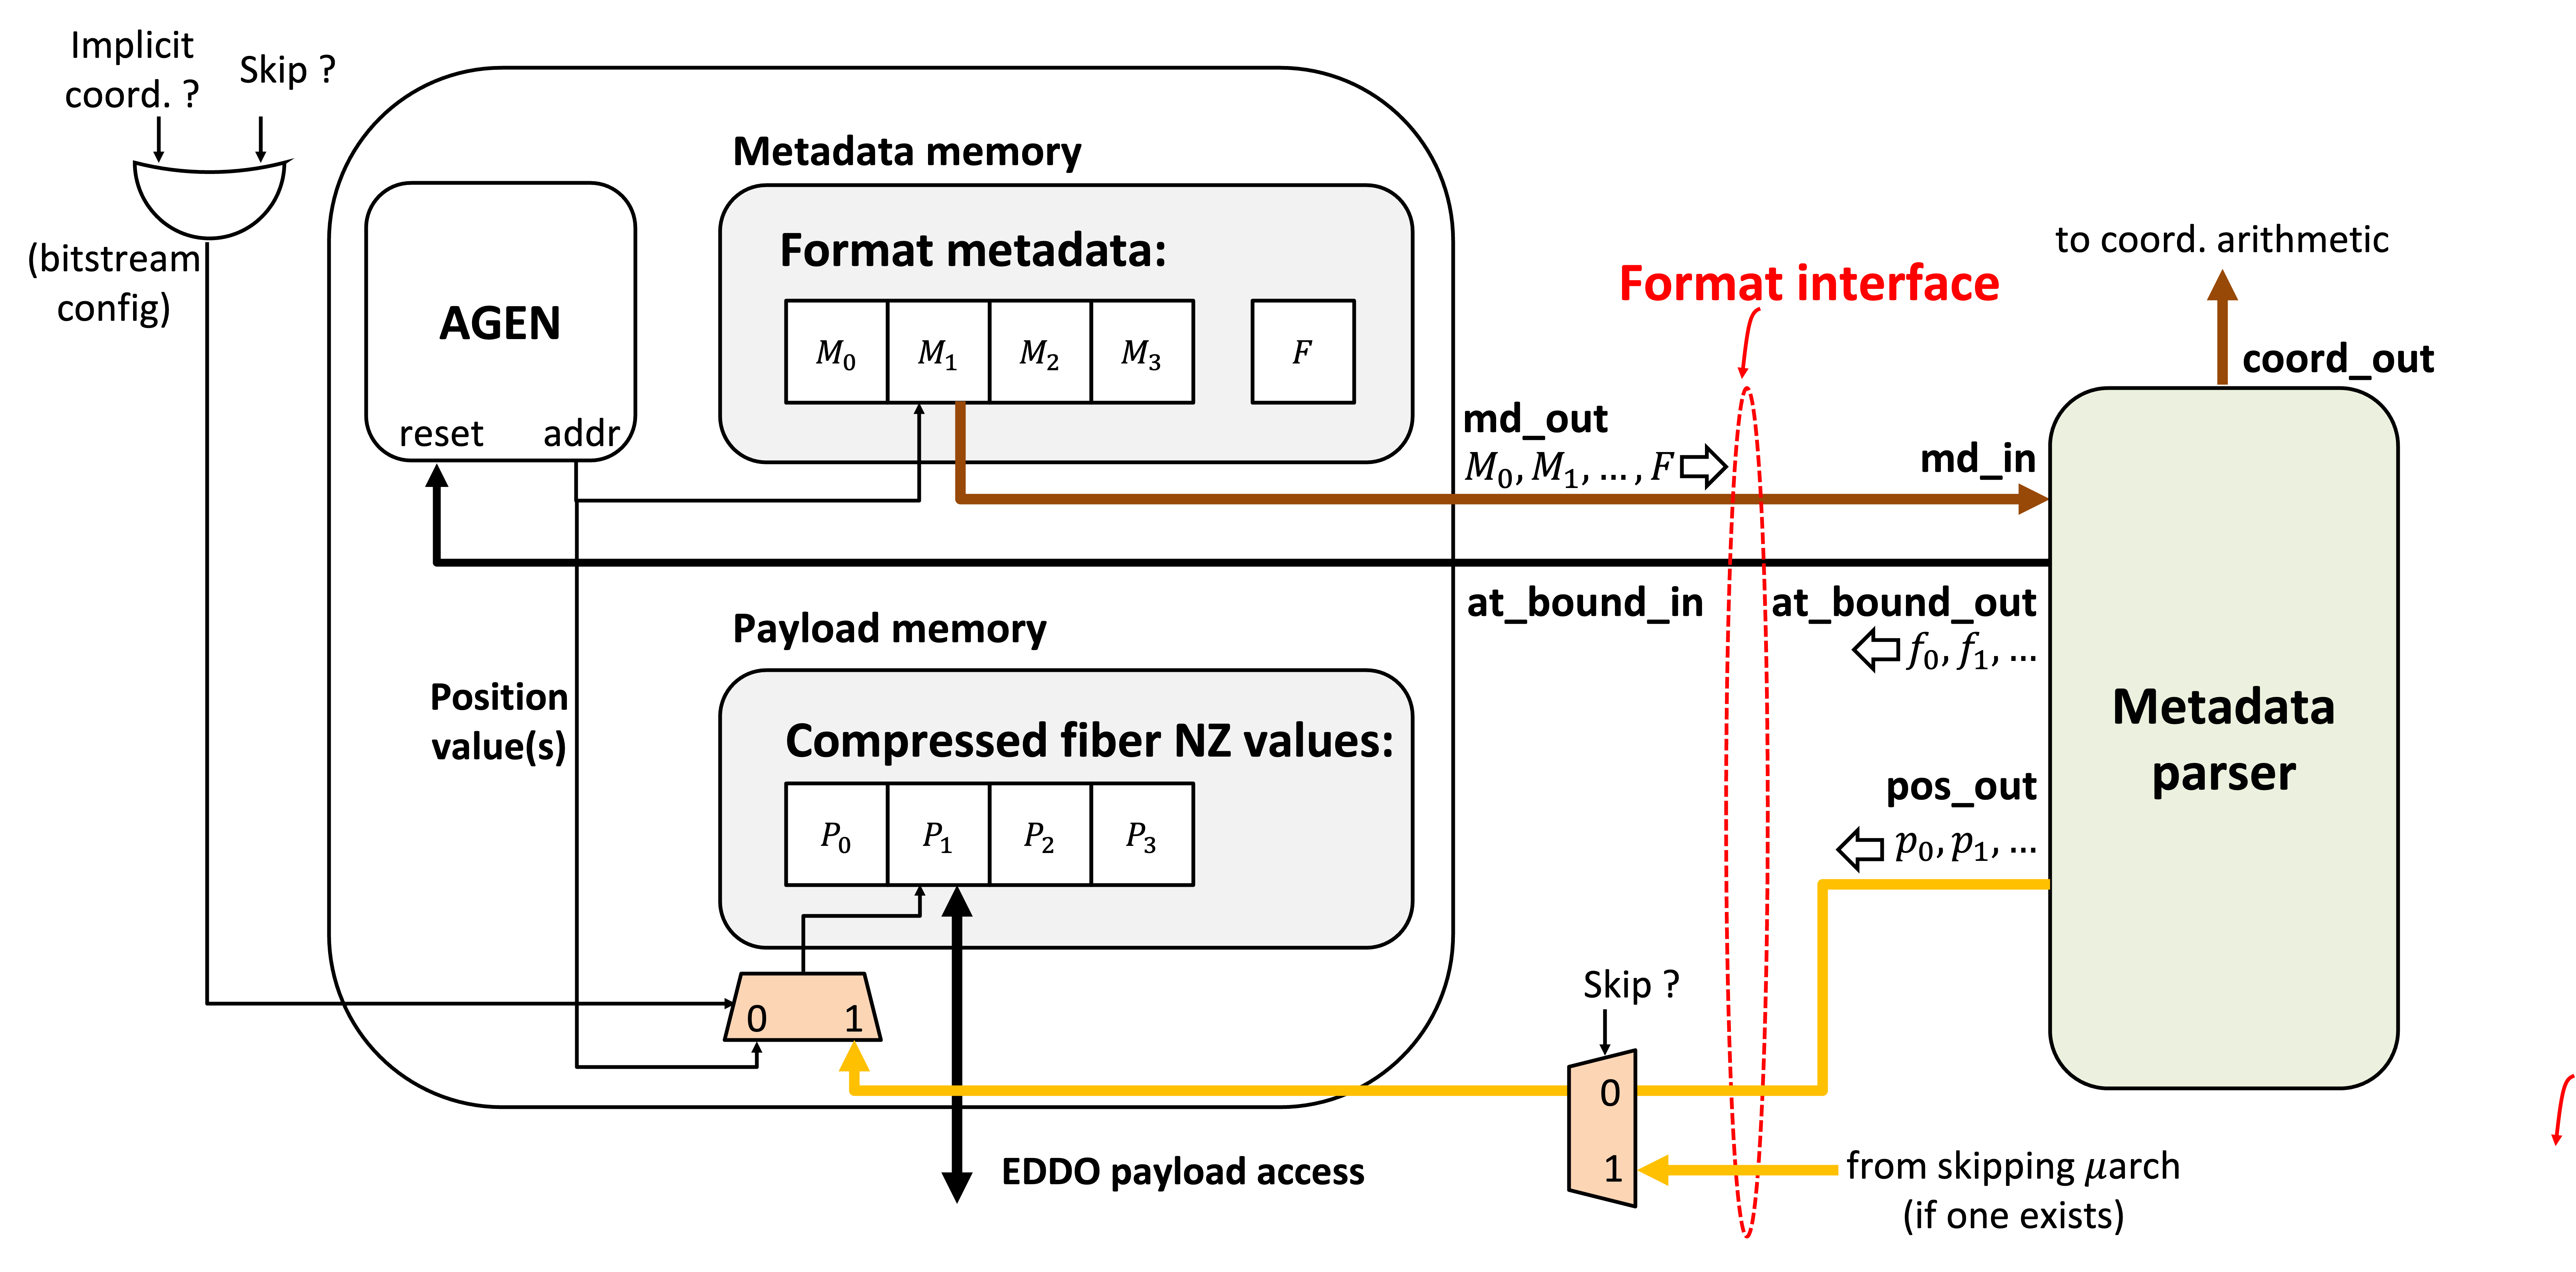
\includegraphics[width=0.95\textwidth]{figures/single_rank_general_format_smartbuffer_model.png}
    \caption{Sparse smartbuffer model for a single rank, supporting general sparse tensor formats. ${M_i}$ are general sparse metadata values, which may not be explicit coordinates. The metadata parser can orchestrate payload reads (via pos\_out) if this is enabled in the configuration bitstream. This is necessary for implicit coordinate representation formats. If skipping is enabled in the configuration bitstream, a skipping microarchitecture's output position stream can orchestrate payload reads. The functionality of the at\_bound\_out signal is unchanged. }
    \label{fig:single_rank_general_format_smartbuffer_model}
\end{figure}

There are a few problems with trying to apply the design in Figure~\ref{fig:single_rank_explicit_coordinate_smartbuffer_model} to a B-formatted fiber:

\begin{itemize}
    \item While B still stores the compressed fiber payloads as a series of consecutive non-zero/non-empty elements, the B-format metadata array always has a length equal to the dense length of the fiber's underlying rank, regardless of the number of non-zeroes. This prevents the AGEN from trivially co-iterating through the format-metadata and compressed-NZ-values arrays, as was done in Section~\ref{sec:single_explicit_fiber}.
    \item The B-format metadata may not be \textit{directly} utilized to lookup into the compressed-NZ-values array, as the metadata does not explicitly contain positional offsets that can be used for the lookup. 
\end{itemize}

In order to even look up into the compressed-fiber-NZ values, Figure~\ref{fig:single_rank_general_format_smartbuffer_model} shows that a different design is required which allows the metadata parser to process the B-format metadata into positional offsets and then request lookups into the compressed-fiber-NZ-values array. It is clear from Figure~\ref{fig:single_rank_general_format_smartbuffer_model} that the format interface bundle described in Section~\ref{sec:single_explicit_fiber} must be augmented with an additional input wire, which can receive requests from the metadata parser to lookup payloads in the compressed-fiber-NZ-values array.

\paragraph{Skipping.} Note that the smartbuffer reference design in Figure~\ref{fig:single_rank_general_format_smartbuffer_model} also optionally supports skipping: the smartbuffer can accept positional read offset values from the skipping microarchitecture, rather than from the metadata parser.

\subsubsection{Multi-rank-pipelined (hierarchical), general-format sparse smartbuffer model}

\begin{figure}[ht]
    \centering
    \includegraphics[width=0.95\textwidth]{figures/hierarchical_general_format_sparse_smartbuffer.png}
    \caption{A sparse smartbuffer that stores a multi-rank tensor, inspired by the ExTensor\cite{extensor} design for traversing and intersecting deep fibertrees. The format microarchitecture implements a rank-parallel metadata processing pipeline. See Figure~\ref{fig:format_interface} for the structure of the format interface I/O bundle.}
    \label{fig:hierarchical_general_format_sparse_smartbuffer}
\end{figure}

\begin{figure}[ht]
    \centering
    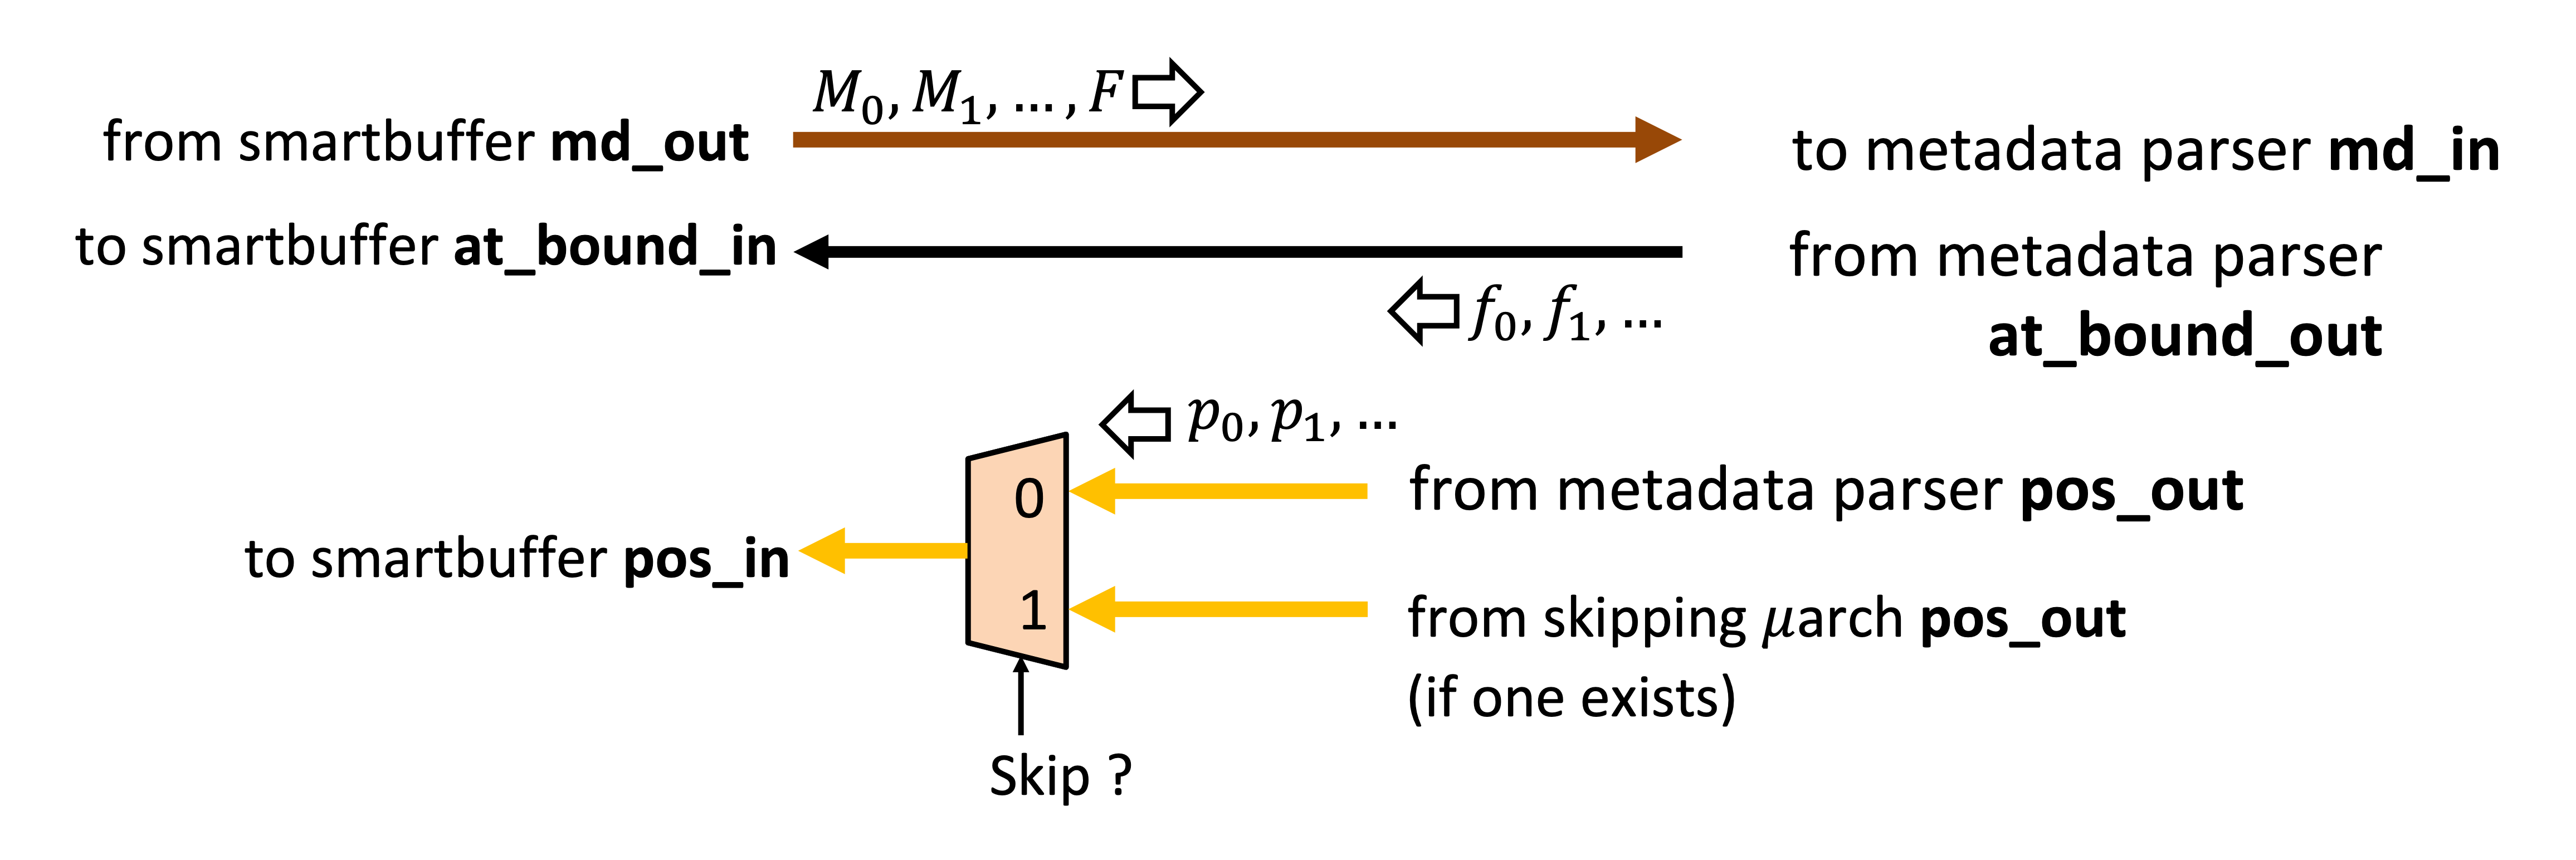
\includegraphics[width=0.95\textwidth]{figures/format_interface.png}
    \caption{Format interface I/O bundle. Sparse metadata moves from md\_out to md\_in. Payload lookup address offsets move from pos\_out to pos\_in. at\_bound\_out signals that fiber traversal is complete. The MUX that switches pos\_in between the metadata parser and the skipping microarchitecture is technically not part of the I/O bundle but is included for clarity and context.}
    \label{fig:format_interface}
\end{figure}

\section{Integrating prior work on skipping microarchitectures}

Previously, a number of papers have introduced microarchitectures which fit the classification of ``skipping microarchitecture'', based on the Sparseloop\cite{sparseloop} definition of skipping (although the authors did not apply this classification themselves.)

This section will:

\begin{itemize}
    \item Propose a unified abstraction for skipping microarchitectures.
    \item Cite Eyeriss v2\cite{eyerissv2} and GAMMA\cite{gamma}, in order to show how leader-follower\cite{sparseloop} skipping microarchitectures may be integrated into the skipping microarchitecture abstraction.
    \item Cite the ExTensor\cite{extensor} and SparTen\cite{sparten} accelerator designs, in order to show how coordinate-payload and bitmask bidirectional skipping microarchitectures may be integrated into the skipping microarchitecture abstraction.
\end{itemize}

\subsection{Unified skipping microarchitecture abstraction}
\label{sec:unified_skipping_abstraction}

\begin{figure}[ht]
    \centering
    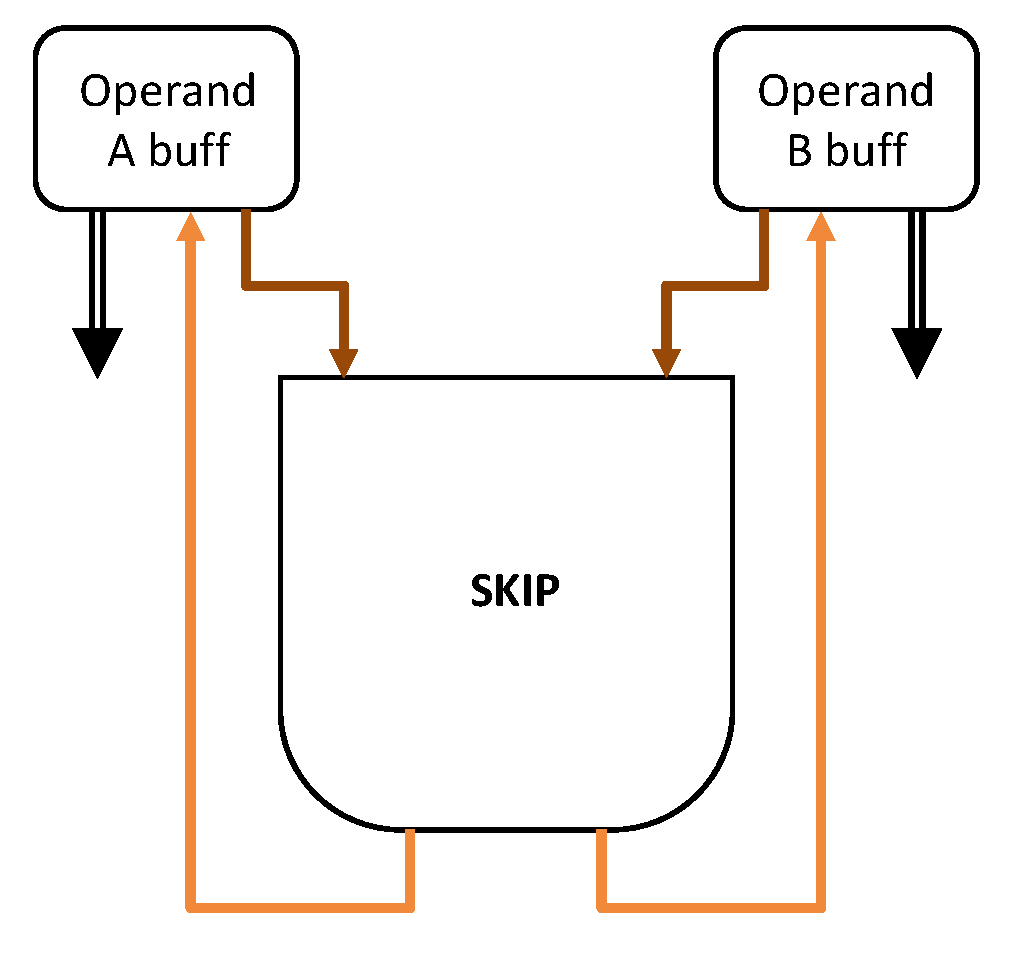
\includegraphics[width=0.7\textwidth]{figures/uniform_skip_topo.pdf}
    \caption{The unified skipping microarchitecture abstraction.}
    \label{fig:uniform_skip_topo}
\end{figure}

Figure~\ref{fig:uniform_skip_topo} shows the unified skipping microarchitecture abstraction developed in this work. The principle of operation is as follows:

\begin{itemize}
    \item Both buffers in Figure~\ref{fig:uniform_skip_topo} are assumed to be co-iterating through compressed sparse fibers along the same rank.
    \item Sparse format metadata is read from each buffer and transmitted to the skipping microarchitecture (\textit{brown wires in} Figure~\ref{fig:uniform_skip_topo}).
    \item Internally, the skipping microarchitecture intersects the sparse format metadata. 
    \item The skipping microarchitecture then - by some means, which is different for each implementation - projects the intersected metadata onto Operand A payload memory address space and Operand B payload memory address space, yielding two streams of positional offsets. These streams of positional offsets effectively select pairs of payloads from the two buffers which have matching coordinates.
    \item The two streams of positional offsets are transmitted to their respective buffers (\textit{yellow wires in} Figure~\ref{fig:uniform_skip_topo}.)
    \item The positional offsets select payloads, which are read from the buffers (\textit{double black lines in} Figure~\ref{fig:uniform_skip_topo}.)
\end{itemize}

Note that this representation of skipping differs from the representation of intersection in \textit{Efficient Processing} (Figure~\ref{fig:efficient_processing_taxo}), because the skipping microarchitecture itself never interacts with payloads; it simply processes sparse format metadata into positional offsets for looking up payloads. 

The following convention will be employed throughout this work: wherever possible, SAF microarchitecture will not directly take payloads as input or produce payloads as output, as doing so would require the SAF microarchitecture to comprehend the details of how payloads are represented, which would dramatically increase the complexity of the abstraction without conveying much additional insight. When a SAF microarchitecture component \textit{must} directly interact with payload streams (as is the case for Fill Optimizers, which will be discussed later in this section), the details of how the component interacts with payloads will be left implicit, i.e. the SAF microarchitecture component will not have explicit input or output ports for payload streams, but will have an annotation that it is bound to a payload stream conceptually.

\subsubsection{Customizing the skipping microarchitecture abstraction for leader-follower skipping}
\label{sec:skipping_lf}

\begin{figure}[ht]
    \centering
    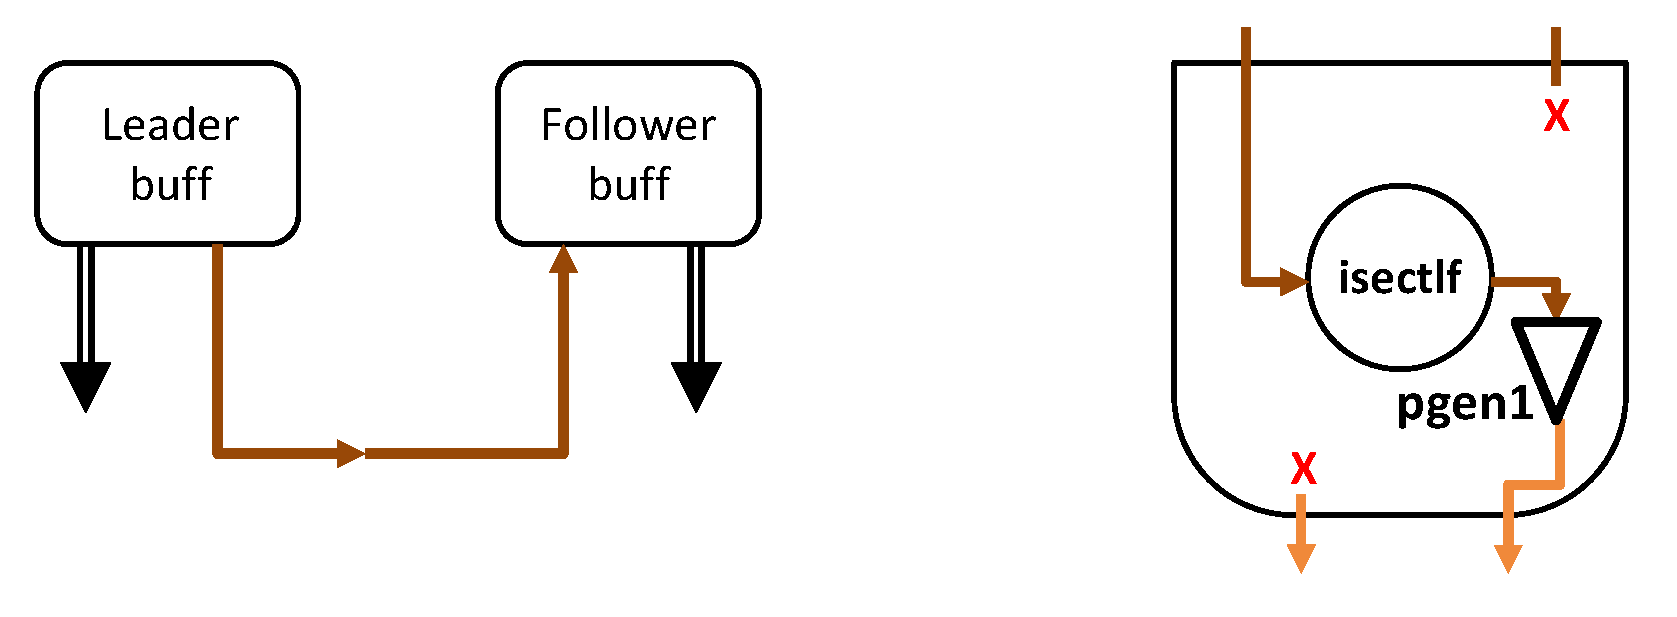
\includegraphics[width=0.7\textwidth]{figures/prior_lf_skip.pdf}
    \caption{\textit{Left:} Leader-follower skipping microarchitectures in prior work (Eyeriss v2\cite{eyerissv2} and GAMMA\cite{gamma}.) \textit{Right:} The skipping microarchitecture abstraction allows ports to be left unused.}
    \label{fig:prior_lf_skip}
\end{figure}

Leader-follower skipping\cite{sparseloop} implements a ``left outer join'' over coordinates; all ``leader'' operand payloads are read from the leader operand buffer, while the sparse format metadata associated with each leader payload is also read and then transmitted to the ``follower'' operand buffer, where the leader metadata is used to lookup and read \textit{only a subset} of follower payloads which match the leader coordinate payloads. 

Sometimes the follower operand will be equal to zero or empty at the coordinate corresponding to the leader payload; in this case, we assume an ineffectual payload is read from the follower buffer.

Figure~\ref{fig:prior_lf_skip} shows how \textit{composition} may be applied in order to customize the skipping abstraction: leader-follower skipping is implemented by a circuit built out of subcomponents connected by wires, which interface with the skipping microarchitecture's input and output ports. Only a subset of the skipping microarchitecture ports (leader-metadata-in a.k.a. \textit{md\_in\_leader} and follower-position-out a.k.a. \textit{pos\_out\_follower}) are utilized, with the other two left unconnected (red X's in Figure~\ref{fig:prior_lf_skip}.)

\paragraph{Coupled data orchestration and coupled position generators in leader-follower skipping.}

Leader-follower skipping exemplifies how SAF microarchitectures may blur the EDDO taxonomy: the skipping microarchitecture is essentially a wire from leader buffer to follower buffer which allows leader metadata to orchestrate follower reads.

It is helpful if we can represent leader-follower skipping microarchitecture in a way that is conceptually consistent with other types of skipping which we will discuss. To that end, the following conventions will be adopted:

\begin{itemize}
    \item \textbf{Skipping always utilizes an intersection unit, even if it is a trivial one.} This will make leader-follower skipping microarchitectures more conceptually consistent with bidirectional skipping microarchitectures, which as we will see can require complex intersection units. We thus introduce a SAF microarchitecture primitive called ``leader-follower intersection'' or \textbf{isectLF} which implements a \textit{trivial intersection}, i.e. a wire directly from operand A buffer to operand B buffer.
    \item \textbf{A \textit{coupled} position generator is always required in order to lookup operand B payloads based on operand A metadata, even if it is a trivial coupled position generator.} In programming languages, it is understood that variables and function arguments may only accept values of matching type. In this work, the abstractions will be more sensible if we require that a wire's datatype must match the datatype of the port it connects to on a buffer or SAF microarchitecture component. Thus, the isectLF may not connect directly to the position input on the operand B buffer, because isectLF outputs a stream of sparse format metadata; the isectLF must connect to a coupled position generator which converts sparse format metadata to a stream of position offsets for looking up operand B payloads. Note that, for the coordinate-payload leader-follower intersections in Eyeriss v2\cite{eyerissv2} and GAMMA\cite{gamma}, it will be a \textit{trivial coupled position generator}, i.e. the position generator will - like the isectLF - be just a wire that passes coordinate metadata unmodified. However, critically, this position generator may not always be trivial - for example, if the leader operand fiber has bitmask (B) metadata and the follower fiber uses uncompressed offset-pair (UOP)\cite{sparseloop} format, then the coupled position generator will need to perform a prefix-sum in order to extract position offsets from the B-format leader metadata. Since the coupled position generator in Figure~\ref{fig:prior_lf_skip} consumes a single metadata stream and outputs a single position offset stream, we will call it a ``single position generator'' or \textbf{pgen1}.
\end{itemize}

One more observation - note that when we describe isectLF and pgen1 as ``trivial'' and as consisting of only a wire from input to output, this is abstracting away the details of pipelining.

\paragraph{Fill optimization.} As was mentioned earlier, a leader operand may trigger an ineffectual payload to be read from the follower buffer. Consider the scenario where the ineffectual payload is an empty fibertree. In this case, the leader operand will be filled into next-level memory or sent to the MAC (depending on the architecture), but there will be no corresponding follower operand. Thus, unnecessary energy, time and memory capacity may be spent operating on the unpaired leader operand.

One approach to handling this scenario, is to simply accept the overhead of unpaired leader operands. Alternatively, existing designs which utilize leader-follower skipping\cite{eyerissv2}\cite{gamma} have means by which to avoid filling unpaired leader tiles into next-level memory (or sending them to MAC). We will refer to this process as ``Fill optimization'' (although the term ``fill'' is somewhat unsuitable for the scenario where the next architectural level is the MAC.)

\begin{figure}[ht]
    \centering
    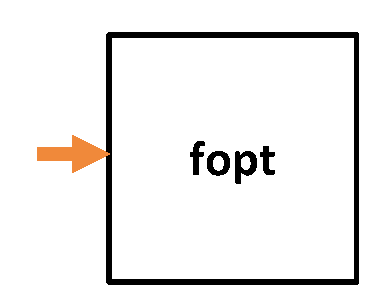
\includegraphics[width=0.6\textwidth]{figures/uniform_fopt.pdf}
    \caption{Unified Fill optimizer (fopt) SAF microarchitecture primitive.}
    \label{fig:uniform_fopt}
\end{figure}

Figure~\ref{fig:uniform_fopt} shows a unified abstraction, developed in this work, for a \textit{Fill optimizer} primitive or \textbf{fopt}. The fopt is implicitly associated with the leader payload stream (recall that by convention SAF microarchitecture components do not have payload I/O's). The fopt takes a position offset input; each position offset selects a position in the payload stream to \textit{keep}; payloads at position offsets which are not explicitly kept, are \textit{discarded} i.e. not filled into next-level memory or sent to the MAC.

Fill optimization may take a number of different forms, and may manifest as either gating of next-level memory fills\cite{eyerissv2}, skipping of next-level memory fills\cite{gamma}\cite{eyerissv2}, or as either gating or skipping depending on the state of the PE pipeline\cite{eyerissv2}. Thus the term ``Fill optimization'' is used to cover all of these eventualities. 

\begin{figure}[ht]
    \centering
    
\includegraphics[width=0.6\textwidth]{figures/leader_lut.pdf}
    \caption{GAMMA\cite{gamma}-style LUT-based Fill optimization.}
    \label{fig:leader_lut}
\end{figure}

Figure~\ref{fig:leader_lut} shows lookup-table-based (LUT-based) Fill optimization as it is employed in GAMMA\cite{gamma}. To be clear, the authors do not use the term ``Fill optimization'' nor do they describe the microarchitecture as performing this function. However, Figure 6\cite{gamma} of the GAMMA paper shows that there is a ``scaling factor register'' file prior to the MAC, which holds leader operand payloads (single data elements); in this work we propose that \textit{one of the functionalities performed by this small memory} - though not necessary its only functionality - is effectively to optimize away unpaired leader payloads. GAMMA reads a stream of leader payloads from main memory, and then (using the Gustavson/row-wise product dataflow\cite{gamma}) triggers loads of follower rows in a leader-follower fashion. In \textit{Efficient Processing} terminology, the follower row would be a fibertree (or sub-tree.) The follower rows enter a merge unit in the PE. Figure 6\cite{gamma} of the GAMMA paper shows that the PE merge unit outputs a stream of (1) ``merged coordinates'' and (2) ``indexes'' associated with the follower fibertree. Given that (1) the merge unit is performing a rank-swap\cite{teaal} and (2) GAMMA employs CSR format for both operands, it is arguable that the stream of indexes represents positional offsets into the uncompressed offset-pair (UOP) rank of the CSR representation of the follower operand. Figure 6\cite{gamma} from GAMMA shows that the indexes from the merger are used to select leader payloads from the scaling factor register; this has a significant implication: if a leader payload is unpaired, then it will never be selected by the indexes-stream from the merge. Thus, the GAMMA PE effectively has a LUT which implements Fill optimization, as shown in Figure~\ref{fig:leader_lut}. This particular Fill optimization would be best described as skipping of unpaired leader fills.

\begin{figure}[ht]
    \centering
    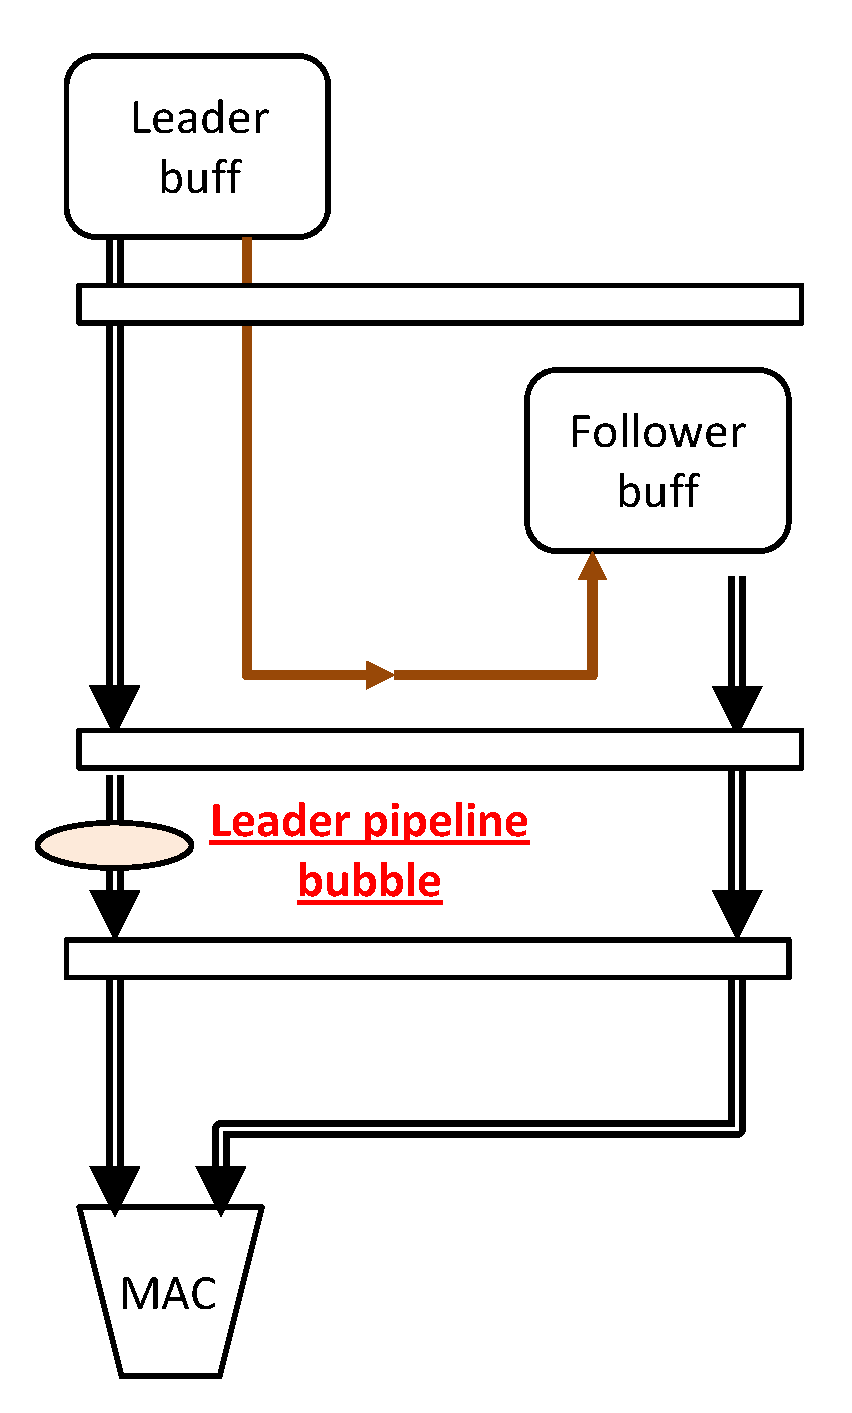
\includegraphics[width=0.6\textwidth]{figures/pipeline_bubble.pdf}
    \caption{Eyeriss v2\cite{eyerissv2}-style pipeline-bubble-based Fill optimization.}
    \label{fig:pipeline_bubble}
\end{figure}

Figure~\ref{fig:pipeline_bubble} shows how pipeline-bubble-based Fill optimization is implemented in Eyeriss v2\cite{eyerissv2}. Eyeriss v2 implements leader-follower skipping in which input activations (iacts) are the leader and weights are the follower. According to \cite{eyerissv2}, ``If there are no non-zero weights corresponding to the non-zero iacts, the non-zero iacts will not be further passed down in the pipeline. This may not necessarily introduce bubbles in the pipeline since the later stages, i.e., after the weight data Spad stage, can still be working on the computation for the previous nonzero iact if it has multiple corresponding weights.'' Note the phrase ``may not necessarily'' - the PE pipeline is effectively managing unpaired leader payloads by introducing a pipeline bubble, and then relying on the latency of downstream pipeline stages to hide the latency introduced by the pipeline bubble. Thus, depending on the degree of latency-hiding which is feasible in practice, the Eyeriss v2 pipeline is either gating or skipping unpaired leader operand fills, as shown in Figure~\ref{fig:pipeline_bubble}.

\subsubsection{Customizing the skipping microarchitecture abstraction for bidirectional skipping}

\begin{figure}[ht]
    \centering
    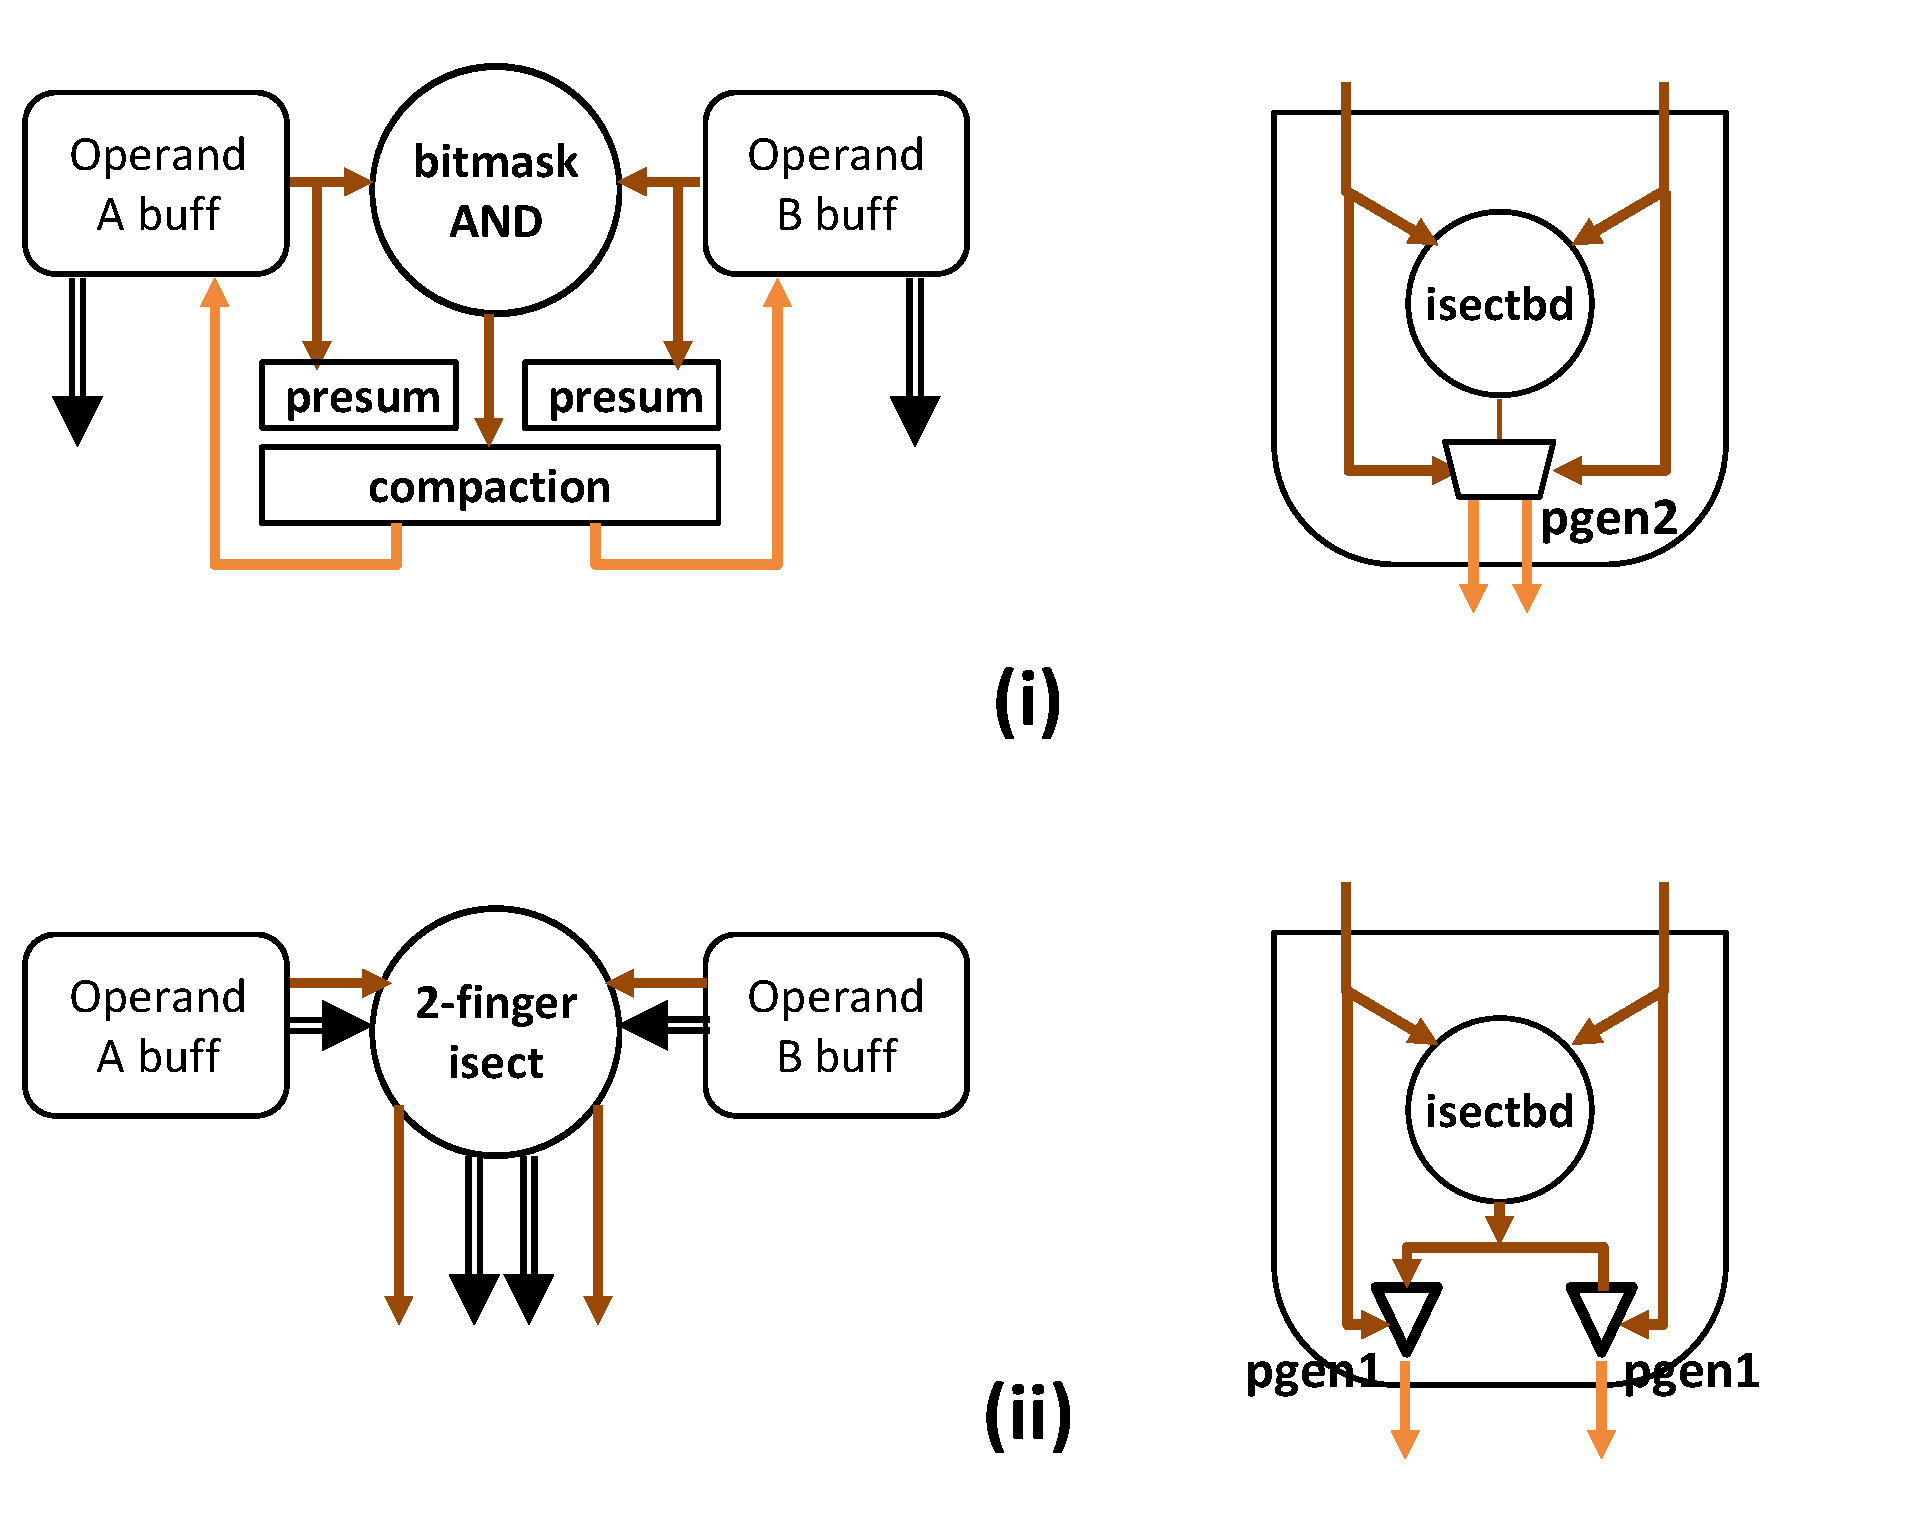
\includegraphics[width=0.95\textwidth]{figures/prior_bd_skip.pdf}
    \caption{Inferring bidirectional skipping microarchitecture topology. (i) \textit{Left:} SparTen\cite{sparten} bitmask(B)-format bidirectional skipping microarchitecture. (ii) \textit{Left:} ExTensor\cite{extensor} naive and optimized coordinate-payload(C)-format bidirectional skipping microarchitectures can be summarized by the same topology. (i) \& (ii) \textit{right:} the B- and C-format bidirectional skipping microarchitectures expressed within the skipping microarchitecture abstraction developed for this work.}
    \label{fig:prior_bd_skip}
\end{figure}

Bidirectional skipping implements an \textit{inner join}; for both operands, only payloads with corresponding coordinates are read. Figure~\ref{fig:prior_bd_skip} shows how bidirectional skipping microarchitectures developed in prior work may be expressed within the skipping microarchitecture abstraction that is developed here. 

Figure~\ref{fig:prior_bd_skip} (i) shows the SparTen\cite{sparten} bidirectional bitmask(B)-format intersection. B-format sparse metadata from both operand buffers is intersected using a bitmask intersection unit; simultaneously, B-format sparse metadata from both operations is prefix-summed in order to compute position offsets for payloads in operand A and operand B memory, respectively. Specialized compaction logic then uses the intersected bitmask metadata to select position offsets from both prefix-sum outputs, compact those position offsets into contiguous vectors, and then stream those position offsets back to the respective operand buffers as payload read requests.

Figure~\ref{fig:prior_bd_skip} (ii) shows the ExTensor\cite{extensor} bidirection coordinate-payload(C)-format intersection (note that this diagram describes both ``naive'' and ``optimized'' extensor intersection units\cite{extensor}.) The intersection process described in ExTensor is more consistent with the \textit{Efficient Processing} view of how intersection works: metadata and payloads go in; only metadata and payloads \textit{corresponding to matching coordinates} come out. However, as described in Section~\ref{sec:unified_skipping_abstraction}, in this work we strive to avoid having SAF microarchitecture directly interact with payload streams. Figure~\ref{fig:prior_bd_skip} (ii) shows how the C-format bidirectional intersection unit may be reorganized and brought into alignment with the unified skipping microarchitecture abstraction developed in this work.

\paragraph{Coupled position generators in bidirectional skipping.}

As shown in Figure~\ref{fig:prior_bd_skip} (i) and Figure~\ref{fig:prior_bd_skip} (ii), the B- and C-format skipping microarchitecture implementations both employ \textit{coupled} position generators.

In Figure~\ref{fig:prior_bd_skip} (ii), the C-format intersection unit consumes and intersects the two input metadata streams, producing a stream of intersected metadata (explicit coordinates common to operands A and B.) The intersected metadata stream is transmitted to two pgen1 units, which output position offset streams for looking up payloads. However, the pgen1 units employed in C-format bidirectional skipping are different from the pgen1 unit employed for leader-follower skipping: these pgen1 units have \textit{reference inputs}, represented in Figure~\ref{fig:prior_bd_skip} as metadata wires going into the side of the pgen1 unit. To understand this, consider the following scenario:

\begin{itemize}
    \item Input A metadata stream: \textbf{0},2,\textbf{3},5
    \item Input B metadata stream: \textbf{0},\textbf{3},6,7
    \item isectBD output stream: 0,3
    \item Left pgen1 output stream (position offsets looking up operand A payloads): 0,2
    \item Right pgen1 output stream (position offsets looking up operand B payloads): 0,1
\end{itemize}

The key insight is, that \textbf{the values of the intersected coordinate payload metadata have no impact on the position offsets used to look up payloads!} Rather, the position offsets for looking up payloads, are derived by finding the \textit{index in the respective input metadata streams} at which the isectBD output metadata values occurred. For example, 3 occurred at position 2 in the Input A metadata stream and position 1 in the Input B metadata stream. 

Thus, the pgen1 units employed in Figure~\ref{fig:prior_bd_skip} (ii) receive the original input metadata stream via the reference input; the primary pgen1 input (the input connected to the isectBD) simply generates an internal event every time a metadata value arrives from isectBD (this is possible if there is a RDY/VLD pipelining scheme.) Every time isectBD raises an event at (for example) the left pgen1 unit, the pgen1 unit outputs the index in the input metadata stream of the most recent metadata value output by isectBD.

Figure~\ref{fig:prior_bd_skip} (i) introduces a new SAF microarchitecture primitive, pgen2. pgen2 or ``dual position generator'' is a coupled position generator which accepts \textit{two} reference metadata streams and outputs \textit{two} position offset streams for looking up payloads. The presence of two reference inputs on pgen2, reflects the observation that both the SparTen B-format skipping microarchitecture and the ExTensor C-format skipping microarchitecture must refer back to the original input metadata streams in order to convert intersected metadata into position offsets. However, in the case of B-format bidirectional intersection, the computation of both position offset streams is grouped into a single pgen2 primitive rather than a pair of pgen1 primitives. The rationale for this grouping is that the prefix sum and compaction logic is not domain-specific to sparse tensor arithmetic; the intermediate output signals produced these components are very implementation-dependent and do not map cleanly onto the \textit{Efficient Processing} datatypes (flag/position/metadata). Thus these operations are all grouped together into the pgen2 unit, which consumes metadata and outpus position offsets. In Figure~\ref{fig:prior_bd_skip} (i), the two metadata reference inputs correspond to the inputs of two prefix-sum units, and the pgen2's primary metadata input (the one connected to isectBD) represented the intersected B-format metadata arriving from bitmask AND.

In this work, it is anticipated that the skipping microarchitecture topologies shown in Figure~\ref{fig:prior_lf_skip} and Figure~\ref{fig:prior_bd_skip}, though described in the context of GAMMA\cite{gamma}/Eyeriss v2\cite{eyerissv2}/SparTen\cite{sparten}/ExTensor\cite{extensor}, could be generalized to describe skipping in a wide range of other published designs, provided that the behaviors of the isectLF/isectBD/pgen1/pgen2 units are customized to reflect these designs.

\section{Overview of conceptual framework proposed in this work}

\begin{figure}[ht]
    \centering
    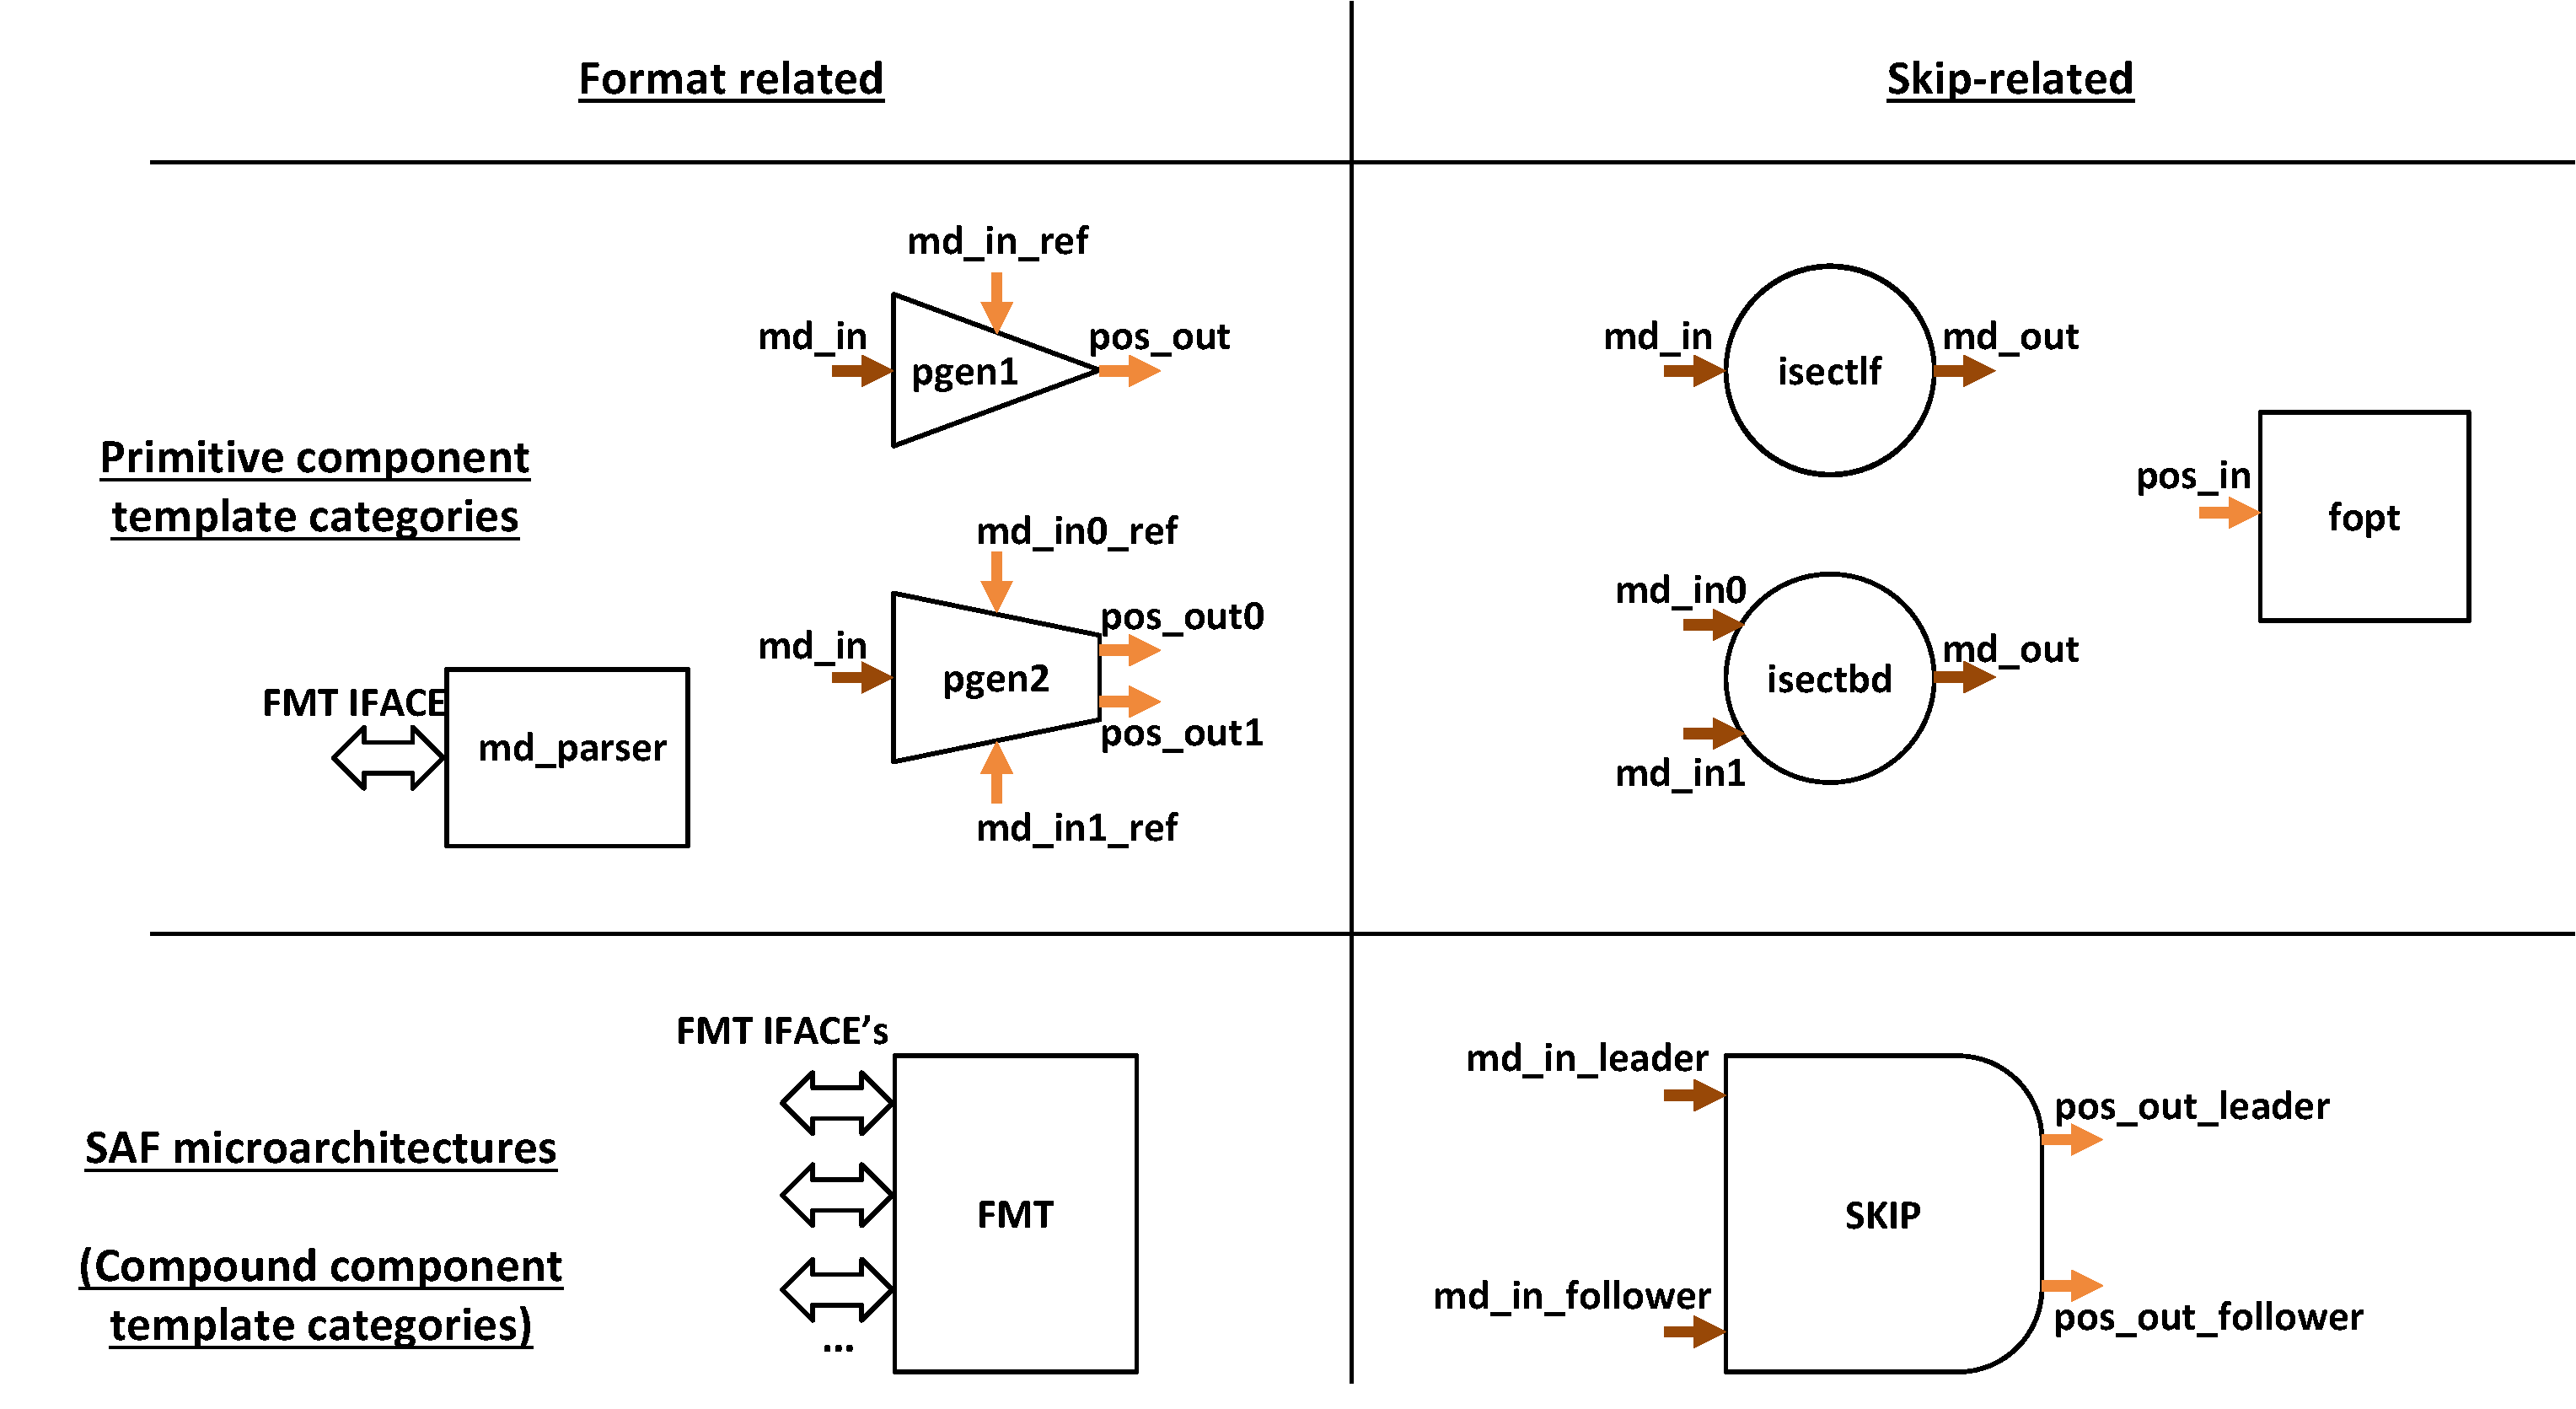
\includegraphics[width=0.95\textwidth]{figures/this_work_taxo.pdf}
    \caption{Overview of the SAF microarchitecture taxonomy developed in this work.}
    \label{fig:this_work_taxo}
\end{figure}

Figure~\ref{fig:this_work_taxo} summarizes the unified taxonomy of format and skipping microarchitecture components developed in this work. The principle of composition is exploited so that a wide range of different format and skipping microarchitecture topologies can be contained with a single consistent format microarchitecture abstraction and a single consistent skipping microarchitecture (Figure~\ref{fig:this_work_taxo}, \textit{bottom}.) Figure~\ref{fig:this_work_taxo} (\textit{top}) summarizes the SAF microarchitecture primitives that can be composed inside of the higher-level format and skipping microarchitecture abstractions, in order to implement a variety of designs. For example,

\begin{itemize}
    \item Metadata parsers (\textbf{mdparser}'s) customized for different sparse representation formats, can be composed with the abstract format microarchitecture (FMT) block, in order to represent sparse format metadata parsing for arbitrary fibertrees. The number of mdparsers can be customized to reflect the depth of the fibertree.
    \item Intersection units (isectLF, isectBD), coupled position generator units (pgen1, pgen2) and fill optimizer (fopt) units may be customized to support different sparse formats and then composed within the abstract skipping microarchitecture (SKIP) block, in order to represent a variety of different skipping microarchitecture designs.
\end{itemize}

In this work, there are three key levels of abstraction:

\begin{itemize}
    \item \textit{SAF microarchitectures/compound components:} These are the highest-level microarchitecture abstractions like SKIP and FMT which are format-agnostic. SAF microarchitecture categories are parameterized by a set of attributes, which determine how the SAF microarchitecture is implemented from SAF microarchitecture primitives.
    \item \textit{SAF microarchitecture primitives:} These components are less abstract and can be customized to handle different sparse representation formats, and can be wired together in abstract circuits in order to implement SAF microarchitectures. Each SAF microarchitecture primitive is associated with an analytical cost model. To facilitate customization, each SAF microarchitecture primitive has a set of \textit{taxonomic attributes}, which select an analytical model appropriate to the particular scenario.
    \item \textit{RTL modules or RTL blocks:} These are not part of the taxonomy introduced in this section; rather, RTL blocks are implemented and characterized in order to obtain metrics on the energy and area costs of specific design choices. RTL blocks are not represented explicitly in SAF microarchitecture designs, but rather their energy/area/timing metrics are referenced when constructing SAF microarchitecture primitive analytical models. Each SAF microarchitecture primitive's analytical model may be constructed from characterized metrics associated with zero or more RTL blocks.
\end{itemize}
